\documentclass{homework}
\usepackage{cancel}
\usepackage{lscape}
\usepackage{xcolor,float}
\usepackage{soul}
\author{Michael D. Walker (mw6136), Philip Satterthwaite (ps1639), Michael Schroeder (ms2774)}
\class{APC523: Numerical Algorithms for Scientific Computing}
\date{\today}
\title{Final Project Report: \href{https://github.com/mw6136/WAVE}{\texttt{WAVE}}\\ Comparing Numerical Methods on Cylindrical Wave Equation Solver Performance}

% Intro 
% General background
% Problem statement
% Contributions
% More deep background
% Methods/Results
%   Philip’s
%   Michael’s
%   Mike’s
% Performance Engineering
% Future Work
% Conclusions/Lessons learned

\begin{document} \maketitle
\section{\textbf{Introduction and Motivation}}
\noindent The ability to understand and predict surface deformation is of great importance to a broad range of applications in fluid dynamics. Particular to our research (lab: \href{https://ctrfl.princeton.edu/}{CTRFL}) are the ocean surface perturbed by wind, and combustion processes (modeled as an iso-surface of fast-reacting chemistry) perturbed by turbulence. Understanding these deformations requires solving high-order partial differential equations, a task that is often impossible to do analytically and must be done numerically.
\begin{figure}[h!]
    \centering
    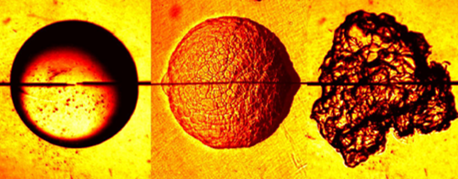
\includegraphics[width = 0.5\textwidth]{media/Law_3_face.png} $\qquad$
    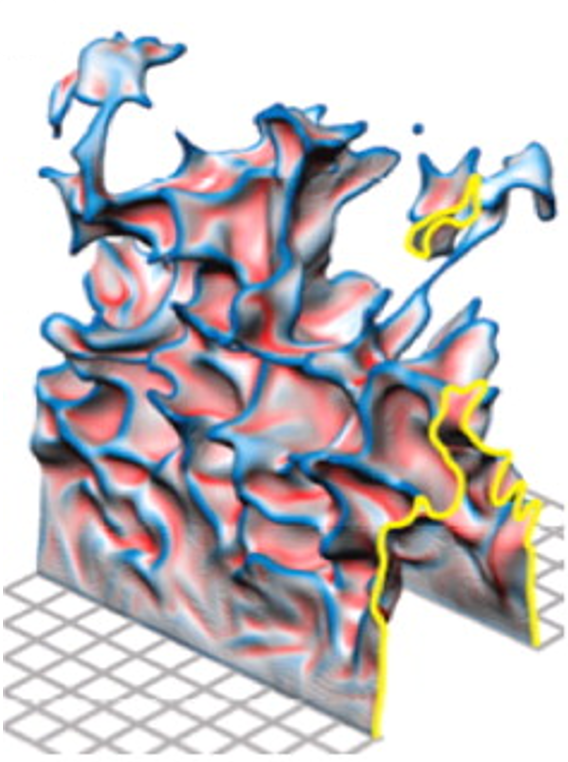
\includegraphics[width = 0.15\textwidth]{media/Driscoll_DNS.png}
    \caption{(left) Increasingly turbulent spherically-expanding flames \cite{Chaudhuri2015}. (right) Direct Numerical Simulation of turbulent Bunsen flames \cite{Driscoll2008}.}
\end{figure}
\\ \noindent
Models of turbulent reacting flows are highly non-linear. Turbulence-chemistry interactions affect virtually every aspect of the flow (there are few passive or conserved scalars). Further, each transport equation requires a model for chemical source term closure. Classically, turbulent flames have been modeled as an ensemble of laminar flamelets, where the turbulent flame is an aggregate of thin, laminar, locally one-dimensional structures present within the turbulent flow field (first done by Williams \cite{Williams_book}, then Peters \cite{Peters_book}). Further, for the case of premixed turbulent combustion, these flames can be simplified using a non-reacting analogue---the $G$-equation. A non-reacting scalar $G$ is modeled according to the level-set equation, thus avoiding complications associated with counter-gradient diffusion and source term closure. $G$ can be considered an iso-scalar surface that divides the flow field into two regions such that $G(x, t) = G_{o}$ can be defined arbitrarily as $G(x, t) > G_{o}$ is the region of burnt gas and $G(x, t) < G_{o}$ is the region of unburnt gas.
\begin{figure}[h]
    \centering
    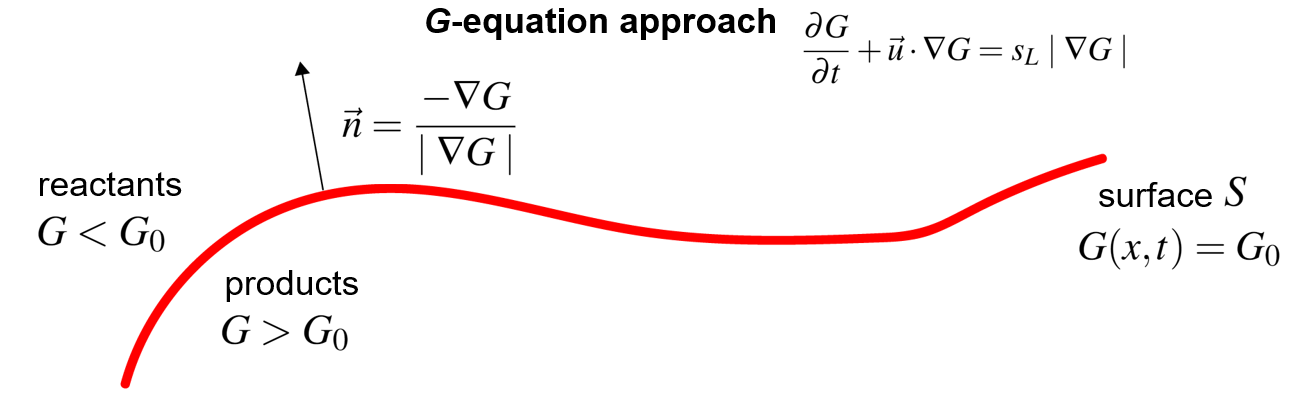
\includegraphics[width = 0.65\textwidth]{media/FSD_G.png}
    \caption{$G$-equation formulation of flame iso-surface.}
\end{figure}
\\ \noindent
The surface then propagates according to level-set equation at the laminar burning velocity $s_L$ in the normal direction $\vec{n} =- \nabla G / |\nabla G|$ at every point on the surface.
$$\frac{\partial G}{\partial t} + \vec{u} \cdot \nabla G = s_{L}|\nabla G|$$
where $\vec{u}$ is the flow velocity field, $| \cdot |$ is the Euclidean norm, and $t$ is time.
\newpage \noindent
While the $G$-equation models the propagation of thin flame structures with a well-defined burning velocity, the flame surface itself (and its deformation due to perturbations by turbulence and chemical heat release) can be modeled according to the scalar wave equation. We seek to build a model of surface deformation by solving the scalar wave equation in cylindrical coordinates. Thereby resolving waves on the surface of a fluid generated by the motion of the walls. Further, we will investigate the trade-offs between speed, cost, accuracy, and stability of various numerical methods.

\begin{figure}[h!]
    \centering
    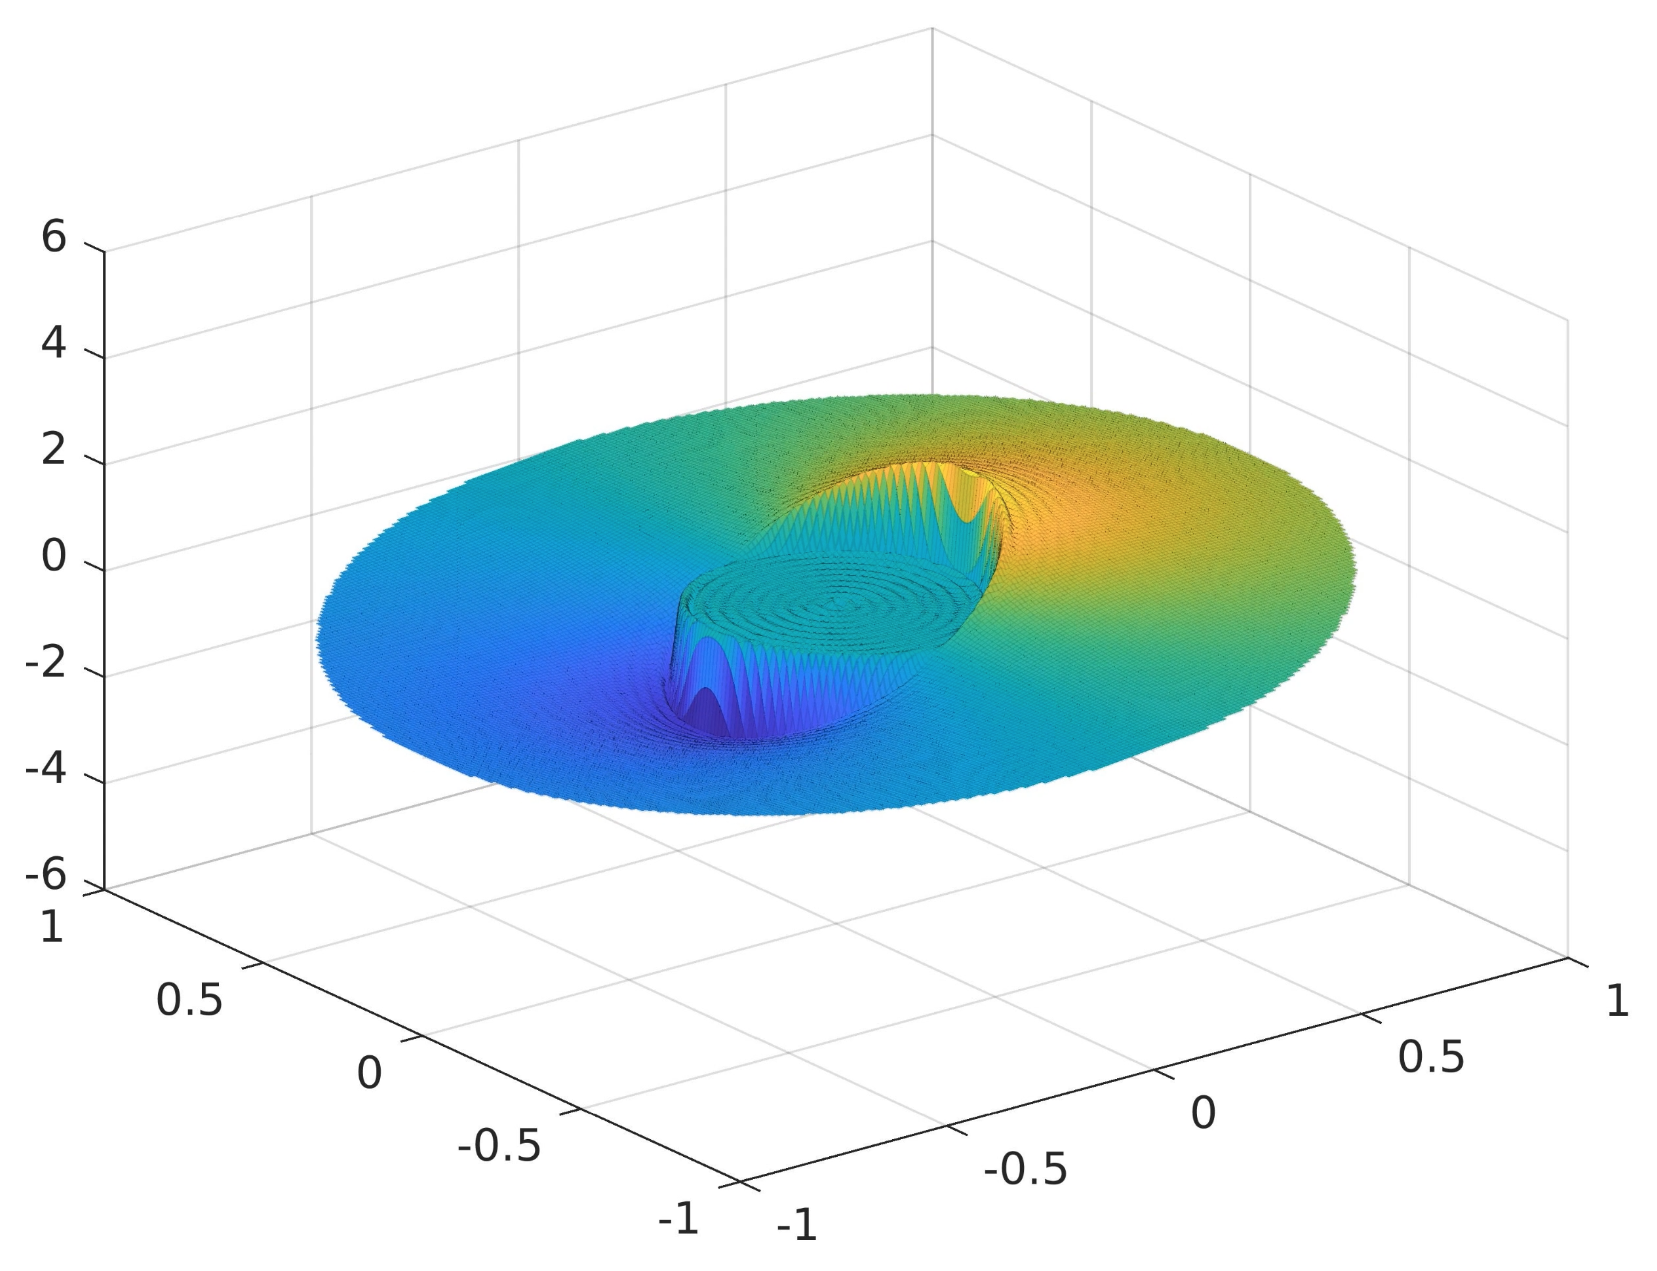
\includegraphics[width = 0.5\textwidth]{media/wave_sol.png}
    \caption{Example solution to the cylindrical wave equation.}
    \label{fig:wave_sol}
\end{figure}
\noindent \textbf{Project Statement} (adapted from \cite{MAE501}) \noindent For a small deformation of any planar circular elastic material, the surface deformation, $\phi$, satisfies the wave equation in plane-polar coordinates
\[ \frac{\partial^2 \phi}{\partial t^2} = c^2 \left[ \frac{1}{r} \frac{\partial}{\partial r} \left(r \frac{\partial \phi}{\partial r}\right) + \frac{1}{r^2} \frac{\partial^2 \phi}{\partial \theta^2} \right]\]
\noindent where the driving force of the wave motion for a material initially at rest can be specified through the boundary and initial conditions. Seeking to model waves on the surface of the fluid generated by the motion of the walls, we choose the following boundary and initial conditions. \\[8pt]
\noindent Boundary Conditions: \\
$ \phi(r=R, \theta, t) = A \cos(\omega t) \cos (\theta) $ \\
$ \phi(r=0, \theta, t) \rightarrow \textrm{finite} $ \\
$ \phi(r, \theta + 2\pi, t) = \phi(r, \theta, t) $ \\[8pt]
\noindent Initial Conditions: \\
$ \phi(r, \theta, t=0) = 0 $ \\
$ \partial \phi/ \partial t \, (r, \theta, t=0) = 0 $
\\[8pt] \noindent
It can be seen that the boundary conditions are ill-posed, but can be re-scaled as a forcing function within a solution to the homogeneous problem. We seek to solve this problem analytically, and through a series of numerical methods discussed below. The Software repository submitted with this report (\href{https://github.com/mw6136/WAVE}{https://github.com/mw6136/WAVE}) contains the scripts for the various numerical approaches, which can be compared using \texttt{run\_cases.py}. Figures were generated with \texttt{Python} and \texttt{MATLAB}.
\\ \\
\noindent \textbf{Michael S. Contributions} 
Michael implemented the analytical solution in \texttt{MATLAB} in both Cartesian and polar coordinate systems. He plotted the solution at a range of timesteps to allow for an easy visual comparison to the numerical solutions. He also created a \texttt{Python} function that can read the exported analytical solution's data and geometry, for use in the numerical methods. He implemented, helped derive, and analyzed the finite difference discretization method. He also analyzed the applicability of iterative methods to this problem. He contributed the relevant sections of this report.
\\ \\
\noindent \textbf{Philip Contributions}
Philip performed the investigation into the time-stepping methods. He wrote the code for the explicit Euler and Runge-Kutta schemes and performed research on the viability of implementing implicit time-stepping schemes. He wrote the relevant sections of the report. 
\\ \\
\noindent \textbf{Michael W. Contributions}
Michael developed the full analytical solution shown in the Appendices (adapted from \cite{MAE501}). He created the \texttt{FFT\_solver} using spectral methods, and further developed improvements in speed and stability, as will be discussed. He contributed the relevant sections of the report, as well as the majority of background, introduction, and conclusion. Most of the presentation slides and the \texttt{README} for documenting and running the code were created by Michael.

\section{\textbf{Analytical and Numerical Methods}}

\subsection{Analytical Solution}
The full derivation of the solution to this problem is shown in Appendix \ref{B}. We solve for $\phi$ for all $t$, $\theta$, and $r$ using the method of separation of variables and eigenfunction expansions. We also determine the resonance condition for the value of $\omega$. 
\\ \\ \noindent
First using separation of variables to de-couple the time component and determine the eigenfunctions for the operator with boundary conditions, we obtain an equation to the radial component that is the Bessel equation, whose solution are the Bessel functions. The angular component takes the form of a classical, 2nd-order undamped ODE, whose solutions are sinusoidal functions. Thus the solution is a linear combination of Bessel and cosine functions for each eigenmode.  The ill-posed boundary conditions can be re-scaled as a forcing function within a solution to the homogeneous problem. The coefficients can then be obtained using the initial conditions and properties of orthogonality.
\\ \\ \noindent
This approach leads to the analytical solution 
$$ \phi(r, \theta, t) = A \left(\frac{r}{R} \right)^2 \cos(\omega t) \cos(\theta) + \tilde{\phi} (r, \theta, t)$$ 

\noindent $\tilde{\phi}$ is composed as follows, where $J_n (\cdot)$ is the Bessel function of the 1st kind and order $n$, $\eta$ is a variable of integration, and $\lambda$ are the eigenfunctions for each of the modes.
$$ \tilde{\phi} (r, \theta, t) = \sum_{m=1}^\infty \Biggl( \frac{1}{c^2 \lambda_{n,m} - \omega^2} \frac{2A}{R^2} \frac{\int_0^1 \left( \omega^2 \eta^2 + 3c^2 \right) \eta J_1\left( \sqrt{\lambda_{1,m}} R \eta \right) d\eta }{{J_2}^2 \left( \sqrt{\lambda_{1,m}} R \right)} \cos(\omega t) \; \dots $$

$$ - \frac{2A}{{J_2}^2 \left( \sqrt{\lambda_{1,m}} R \right)}\Bigg[ \int_0^1 \eta^3 J_1 \left( \sqrt{\lambda_{1,m}} R\eta \right) d\eta \; \dots $$

$$ + \frac{1}{c^2 \lambda_{n,m} - \omega^2} \frac{1}{R^2} \int_0^1 \left(\omega^2 \eta^2 + 3c^2 \right) \eta J_1 \left(\sqrt{\lambda_{1,m}} R \eta \right) d\eta \Bigg] \cos \left(c \sqrt{\lambda_{1,m}} t \right) \Biggl) \cos(\theta) J_1 \left(\sqrt{\lambda_{1,m} } r \right) .$$

\noindent By inspection of $\tilde{\phi}(r, \theta, t)$, the coefficient in the summation goes to infinity and ``blows up'' as the denominator $c^2 \lambda_{n,m} - \omega^2 \rightarrow 0$, thus a resonance condition exists when $c^2 \lambda_{n,m} = \omega^2$. Recall that $\lambda_{n,m}$ is the eigenmode for the $m$-th root of the $n$-th order Bessel function $J_n$ for $m = 1,2,3 \dots$. Thus, $c \sqrt{\lambda_{n,m}}$ can be interpreted as an eigenfrequency which, when excited, results in resonance.
\newpage
\subsection{Finite Difference Discretization}

\subsubsection{\textbf{Analytical Derivation}}
To discretize the wave equation in polar coordinates \cite{StackEx}, define $r = i \Delta r$, $\theta = j \Delta \theta$, and $t = n \Delta t$. Thus,
$$ \phi \left(r, \theta, t \right)= \phi \left(i \Delta r, j \Delta \theta, n \Delta t \right) = \phi \left(r_i, \theta_j, t^{\left(n\right)} \right) \equiv \phi_{i,j}^{\left(n\right)} $$
where $r_i$ and $\phi_j$ are the positions and $\Delta r$ and $\Delta \theta$ are the cell widths.
\\[5pt] \noindent
Considering the Laplacian is divergent at $r=0$:
$$ \nabla^2 = \frac{1}{r} \, \frac{\partial}{\partial r} \left(r \frac{\partial}{\partial r}\right)+ \frac{1}{r^2} \frac{\partial^2}{\partial \theta^2} $$
so too will the discretization diverge. This can be managed in several ways.
\begin{itemize}
    \item Choose a problem such that $r=0$ does not need to be considered (e.g., $r_{\textrm{min}} = 0.001$). This is usually the method we employ. 
    \item Use cell-centered values for $r$ (e.g., $r_{\textrm{min}} = 0.5 \Delta r$)
    \item Use two meshes: a Cartesian one for $r  \leq 1$ and a polar one for $r \geq 1$, merging them at $r \simeq 1 $ (requires at least 1 cell of overlap).
\end{itemize}

\noindent Using the forward difference in $r$ and central differences in $\theta$ and $t$,
\begin{align*}
    \frac{1}{r} \, \frac{\partial}{\partial r}\left(r \frac{\partial \phi}{\partial r} \right) &= \frac{1}{r_i} \left(r_{i+1/2} \frac{\phi^{\left(n\right)}_{i+1,j} - \phi^{\left(n\right)}_{i,j}}{\Delta r^2} - r_{i-1/2} \frac{\phi^{\left(n\right)}_{i,j} - \phi^{\left(n\right)}_{i-1,j}}{\Delta r^2} \right) \\
    \frac{1}{r^2} \frac{\partial^2\phi}{\partial \theta^2} &= \frac{1}{{r_i}^2} \left( \frac{\phi^{\left(n\right)}_{i,j+1} - 2 \phi^{\left(n\right)}_{i,j} + \phi^{\left(n\right)}_{i,j-1}}{{\Delta \theta}^2} \right) \\
    \frac{\partial^2 \phi}{\partial t^2} &= \frac{\phi^{(n+1)}_{i,j} - 2 \phi^{(n)}_{i,j} + \phi^{(n-1)}_{i,j}}{\Delta t^2}
\end{align*}
\\ \noindent
where $r_{i + 1/2}= 0.5 \left(r_{i+1} + r_i \right)$ and $r_{i - 1/2}= 0.5 \left(r_i + r_{i-1} \right)$. Thus the full wave equation becomes
$$
\phi^{(n+1)}_{i,j} = \Delta t^2 c^2 \left[ \frac{1}{r_i} \left(r_{i+1/2} \frac{\phi^{\left(n\right)}_{i+1,j} - \phi^{\left(n\right)}_{i,j}}{\Delta r^2} - r_{i-1/2} \frac{\phi^{\left(n\right)}_{i,j} - \phi^{\left(n\right)}_{i-1,j}}{\Delta r^2} \right) + \frac{1}{{r_i}^2} \left( \frac{\phi^{\left(n\right)}_{i,j+1} - 2 \phi^{\left(n\right)}_{i,j} + \phi^{\left(n\right)}_{i,j-1}}{{\Delta \theta}^2} \right) \right] + 2 \phi^{(n)}_{i,j} - \phi^{(n-1)}_{i,j}
$$
% \begin{align*}
%     \phi_{i,j}^{\left(n+1\right)} &= 2 \phi_{i,j}^{\left(n\right)} - \phi_{i,j}^{\left(n-1\right)} \\
%     &+ \frac{c^2 \Delta t^2}{\Delta r^2}\left[\phi_{i+2,j}^{\left(n\right)} + \frac{1}{i}\phi_{i+2,j}^{\left(n\right)} - 2\phi_{i+1,j}^{\left(n\right)} - \frac{1}{i}\phi_{i+1,j}^{\left(n\right)} + \phi_{i,j}^{\left(n\right)}\right] \\
%     &+ \frac{c^2 \Delta t^2}{i^2 \Delta r^2 {\Delta \theta}^2} \left[\phi_{i,j+1}^{\left(n\right)} + \phi_{i,j-1}^{\left(n\right)} - 2\phi_{i,j}^{\left(n\right)} \right]
% \end{align*}
\\ \noindent
The spatial discretization is $\Delta r$, $\Delta \theta$ is user defined. The timestep $\Delta t$ is limited by the Courant-Friedrichs-Levy (CFL) condition. For the wave equation, such that
$$ c^2 \frac{\Delta t}{\min(\Delta r^2, {\Delta \theta}^2)} \leq \frac{1}{2} $$
Where formally the constant is limited by the dimensionality of the system $ 1 / N_{\textrm{dim}}$. For time-stepping purposes, this is the speed limitation of the algorithm. Thus, for performance, it is worthwhile to consider Implicit methods.

\subsubsection{\textbf{Numerical Implementation}}
This method was implemented to solve the project's problem statement. Since we already had access to the analytical solution, we knew that $\phi(r=0, \theta, t) = 0$, and so this was used to eliminate the divide by zero error. This, and the fact that there is a prescribed boundary condition allowed us to never consider the ill-posed quantities $r_{0-1/2}$ and $r_{N+1/2}$.


\subsection{\textbf{Iterative Methods}}
Simple iterative methods solve the system $\mathbb{A} \mathbf{u} = \mathbf{b}$. They are useful when $\mathbb{A}$ is hard to invert, and they work by decomposing $\mathbb{A}$ into $\mathbb{A} = \mathbb{M} - \mathbb{N}$, where $\mathbb{M}$ is easy to invert, and then iteratively solving for $\mathbf{u}^{n+1} = \mathbb{M}^{-1} \mathbb{N} \mathbf{u}^n + \mathbb{M}^{-1} \mathbf{b}$.

\subsubsection{\textbf{Jacobi Iteration}}
In the Jacobi method, iterate using $\mathbb{M} = \text{diag}(\mathbb{A})$ and $\mathbb{N} = \text{diag}(\mathbb{A}) - \mathbb{A}$.

\subsubsection{\textbf{Gauss-Seidel Iteration}}
In a Gauss-Seidel iterative scheme, iterate using $\mathbb{M} = \text{diag}(\mathbb{A}) + \mathbb{L}$ and $\mathbb{N} = - \mathbb{U}$.

\subsubsection{\textbf{Successive Over-Relaxation}}
In Successive Over-Relaxation (SOR), the Gauss-Seidel iteration is first calculated, then an over-relaxation parameter $\omega$ is defined and varied to determine the optimal value for the given set of equations. It is implemented as $u_i^{n+1} = u_i^n + \omega (u_i^{GS} - u_i^n)$.

\subsection{\textbf{Time-Stepping Methods}}
\noindent These methods discretize the time domain into small intervals and approximate the solution at each timestep. They iteratively advance the solution from an initial condition to a desired final time, updating the solution at each timestep based on the governing equations. Using a grid of 100 discretizations in both radial and azimuthal directions and a time-step of $\Delta t = 5\cdot 10^{-4}$, the following methods were used to estimate the solution to $\phi$ at time $t = 0.5$.

\subsubsection{\textbf{Forward Euler}}
The forward Euler method is a numerical technique for solving ordinary differential equations by approximating the solution at the next timestep based on the derivative at the current timestep, often used for its simplicity but limited by its first-order accuracy and potential stability issues.
\\ \\ \noindent
Through a series of numerical differentiations, the second derivative of the wave equation can be approximated. The second derivative with respect to $r$ can be expressed as
\[ \frac{1}{r} \frac{\partial}{\partial r} \left(r \frac{\partial \phi}{\partial r}\right) = \frac{\phi \left( r+dr,\theta \right) - 2\phi \left( r,\theta \right) + \phi \left( r-dr,\theta \right)}{dr^2}\]
for any $r$. Similarly, the second derivative with respect to $\theta$ is
\[ \frac{1}{r^2} \frac{\partial^2 \phi}{\partial \theta^2} = \frac{\phi \left( r,\theta+d\theta \right) - 2\phi \left( r,\theta \right) + \phi \left( r,\theta-d\theta \right)}{{d\theta}^2}\]
Thus, with a known value for $c$, the second derivative of $\phi$ with respect to time is known.
\\ \\ \noindent
With known initial conditions, we can progress through the time steps and calculate $\phi ^{n+1}$. Since the value which we have calculated is merely a change in the second-order relationship, we must use a second-order forward Euler scheme:
\[
\phi ^ {(n+1)} = \phi^{(n)} + (\phi^{(n)}-\phi^{(n-1)} ) \Delta t +\Delta t^2\frac{\partial^2 \phi}{\partial t^2}
\]
where $\phi^{(n)}-\phi^{(n-1)}$ represents the linear change and $\Delta t^2\frac{\partial^2 \phi}{\partial t^2}$ is the second-order change.

\subsubsection{\textbf{Backward Euler}}
This method is implicit, so the solution at the next timestep is approximated based on the derivative at the future timestep. Unlike forward Euler, it is unconditionally stable but is more computationally expensive. For this three dimensional wave equation, the implicit Euler method is not a viable scheme. As this method relies on a root-finder to determine a solution for the next time step, it is relatively efficient for equations with one dimensional variation in space. Since the equation we are solving varies in two dimensions, one would need to solve an $N^2$ non-linear system of equations for each time step to fully resolve the solution. This would come with largely increased computational cost for the sole benefit of having better stability than the forward Euler method. As will be shown in Section 3.3, the explicit scheme converged, so the development of the implicit Euler method would be superfluous.

\subsubsection{\textbf{Runge-Kutta}}
This method iteratively approximates the solution at each timestep using a weighted average of multiple intermediate slopes. It is significantly more accurate than other similar methods.
\\ \\ \noindent
Due to the added complexity of the higher-dimensionality of this problem, only the RK2 method was implemented. In this method, the second-order derivative term is calculated twice. The first time is the same as outlined in the forward Euler method (2.4.1). This is then used to estimate $\phi^{(n+\frac{1}{2})}$, where the second-order variation is calculated to a higher accuracy and used to calculate $\phi^{(n+1)}$. It is expected that this method will produce results with a higher level of precision than the Euler method.

\subsection{\textbf{Fourier Spectral Methods}} Spectral methods are employed for solving differential equations by representing the solution as a sum of basis functions. They offer high accuracy and convergence rates, making them particularly suited for problems with smooth solutions or periodic boundary conditions. Fourier series represent periodic functions as an infinite sum of sinusoidal functions. By expanding the solution in terms of Fourier modes, spectral methods can efficiently capture periodic behavior and rapidly converge to the solution, especially for problems with periodic boundary conditions such as ours.
\\ \\ \noindent
The wave equation in the frequency domain can be derived by taking the Fourier transform of the wave equation in the spatial domain. A 2-D Fourier transform in polar coordinates is defined as 
$$ \mathcal{F}(k_r, k_\theta) = \int_0^\infty \int_{-\pi}^\pi f(r, \theta) \exp(-i r k_r \cos(k_\theta - \theta)) r \, dr d\theta $$
\noindent
where $k_r$ and $k_\theta$ are the spatial frequency radius and angle. The corresponding 2-D inverse Fourier transform is written
$$ f(r, \theta) = \frac{1}{(2 \pi)^2} \int_0^\infty \int_{0}^{2\pi} \mathcal{F}(k_r, k_\theta) \exp(i \langle k_r, k_\theta \rangle \cdot \langle r, \theta \rangle) r \, d k_r \, d k_\theta $$
\noindent
Therefore the Fourier pair for the 2-D Laplacian in polar coordinates \cite{Baddour2011, Costa2004}
$$ \nabla^2 f(r, \theta) = \frac{\partial^2 f}{\partial r^2} + \frac{1}{r} \frac{\partial f}{\partial r} + \frac{1}{r^2} \frac{\partial^2 f}{\partial \theta^2} \quad \longleftrightarrow \quad {k_r}^2 \mathcal{F}(k_r, k_\theta) + \frac{{k_{\theta}}^2}{r^2} \mathcal{F}(k_r, k_\theta) .$$
\noindent
By applying the temporal Fourier transform to the scalar wave equation in polar coordinates, the RHS becomes a simple algebraic relation, where $\mathcal{F}(\phi) \equiv \hat{\phi}$. To transform this equation into the frequency domain, we take the Fourier transform of both sides with respect to the spatial coordinates $r$ and $\theta$, while keeping time $t$ unchanged. The Fourier transform of a derivative is given by multiplication by the corresponding frequency---greatly simplifying the calculation of the Laplacian. The wave equation in the frequency domain becomes:
$$ \frac{{\partial^2 \phi}}{{\partial t^2}} = c^2 \left[ \frac{1}{r} \frac{\partial}{\partial r} \left(r \frac{\partial \phi}{\partial r}\right) + \frac{1}{r^2} \frac{\partial^2 \phi}{\partial \theta^2} \right] \quad \longleftrightarrow \quad \frac{{\partial^2 \hat{\phi}}}{{\partial t^2}} = -c^2 \left( {k_r}^2 \hat{\phi} + \frac{{k_{\theta}}^2}{r^2} \hat{\phi} \right).$$
\noindent
This equation governs the evolution of the Fourier components of the solution $\hat{\phi}$ with respect to time $t$. Mathematically, this is the \emph{Helmholtz differential equation} in polar coordinates, which represents a time-independent form of the wave equation. In 1-D it is a linear PDE that takes the form of a strict eigenvalue problem $ \nabla^2 f = -k^2 f$ with $k^2$ an eigenvalue (the wave number) and $f$ the eigenfunction.
\\ \\ \noindent
The time forcing term $\partial^2 \hat{\phi} / \partial t^2$ can then progress through an iterative scheme. Here, the forward Euler equation is chosen as it is the simplest iterative scheme to implement. In polar coordinates, the discretized finite differences would be as follows:
$$ \phi_{i,j}^{(n+1)} = 2 \phi_{i,j}^{(n)} - \phi_{i,j}^{(n-1)} + \left( \Delta t \right)^2 \left( c^2 \left[ \frac{1}{r_i} \frac{\partial}{\partial r} \left( r_i \frac{\partial \phi}{\partial r} \right) + \frac{1}{r_i^2} \frac{\partial^2 \phi}{\partial \theta^2} \right] \right)^{(n)},$$
\noindent
where $\phi_{i,j}^{(n)}$ represents the value of $\phi$ at radial grid point $r_i$, angular grid point $\theta_j$, and timestep $t^n$ ($\Delta t$ is the timestep size). This equation updates the solution at each timestep based on the values at the previous timestep and the spatial derivatives of the solution. The equation for updating \( \hat{\phi} \) in frequency domain is:
$$ \hat{\phi}^{(n+1)} = 2 \hat{\phi}^{(n)} - \hat{\phi}^{(n-1)} + (\Delta t)^2 \left[ -c^2 \left( {k_r}^2 + \frac{{k_{\theta}}^2}{r^2} \right) \right] \hat{\phi}^{(n)} . $$
\noindent
This process allows the evolution of the solution in the frequency domain over time, and can then be transformed back to the time domain with the inverse $\mathcal{F}^{-1}(\hat{\phi}) = \phi$. The discrete Fast Fourier Transform (FFT) is computed using the \texttt{SciPy} package in \texttt{Python}. First $k_r$ and $k_\theta$ sample frequencies are computed from the $r_i$, $\theta_j$ discretization using \texttt{fftfreq}. Then the transformed Laplacian is computed algebraically and $\hat{\phi}^{(n)}$ is updated according to the forward Euler scheme, then transformed back into the spatial domain with \texttt{ifft}.
\begin{lstlisting}[language=Python]
# Calculate frequencies
freq_r = fftfreq(num_r, dr)
freq_theta = fftfreq(num_theta, dtheta)

# Calculate Laplacian in frequency domain
k_r_squared = (2 * np.pi * freq_r) ** 2
k_theta_squared = (2 * np.pi * freq_theta) ** 2
laplacian = -c ** 2 * (k_r_squared[:, np.newaxis] + k_theta_squared)

# Update phi in frequency domain using forward Euler
phi_hat_next = 2 * phi_hat_curr - phi_hat_prev + dt ** 2 * laplacian * phi_hat_curr

# Transform back to spatial domain
phi_next = np.real(ifft(phi_hat_next, axis=0))
\end{lstlisting}

\section{\textbf{Results}}

\subsection{\textbf{Finite Difference Discretization}}
This method proved fast and accurate, as can qualitatively be seen in Figure \ref{big}. For the utilized $\Delta r$ and $\Delta \theta$, the CFL condition suggests a maximum $\Delta t$ of about $1.3\cdot 10^{-5}$. However, running the simulation and varying $\Delta t$ showed that, at least for $0\leq t \leq 100$, the system is stable for $\Delta t \lesssim 1.5 \cdot 10^{-4}$.
\\ \\ \noindent
Figure \ref{MSE_all} shows the mean square error (MSE) of this numerical method versus the analytical solution, with varying timesteps. All of the cases with $\Delta t \leq 1.5 \cdot 10^{-4}$ line up nearly identically, showing that all of them converge and are fine timestep choices. The code that ran this simulation was parallelized with \texttt{Numba} and ran on 10 cores in the Princeton \texttt{Adroit} cluster. The runtimes were 30 seconds for $\Delta t = 10^{-4}$, 1 minute 59 seconds for $\Delta t = 10^{-5}$, and 16 minutes 4 seconds for $\Delta t = 10^{-6}$. This emphasizes the fact that simulations should generally use the largest stable timestep. Three datapoints is not a lot, but these three points satisfy the scaling relation runtime $\sim \Delta t ^{-1}$.
\\ \\ \noindent
MSE is plotted rather than other error metrics because it best captures the fact that this method is quite similar to the actual solution, as is qualitatively shown in Figure \ref{big}. For example, L2 errors sum up over all $N^2=40,000$ points, making its value high even though the results are similar. 
\begin{figure}[h!]
    \centering
    \includegraphics[width = 0.75\textwidth]{media/big_comparison.png}
    \caption{Visual comparison between the numerical solution ($\Delta t = 10^{-4}$) and analytical solution at four times.}
\label{big}\end{figure}
\begin{figure}[H]
    \centering
    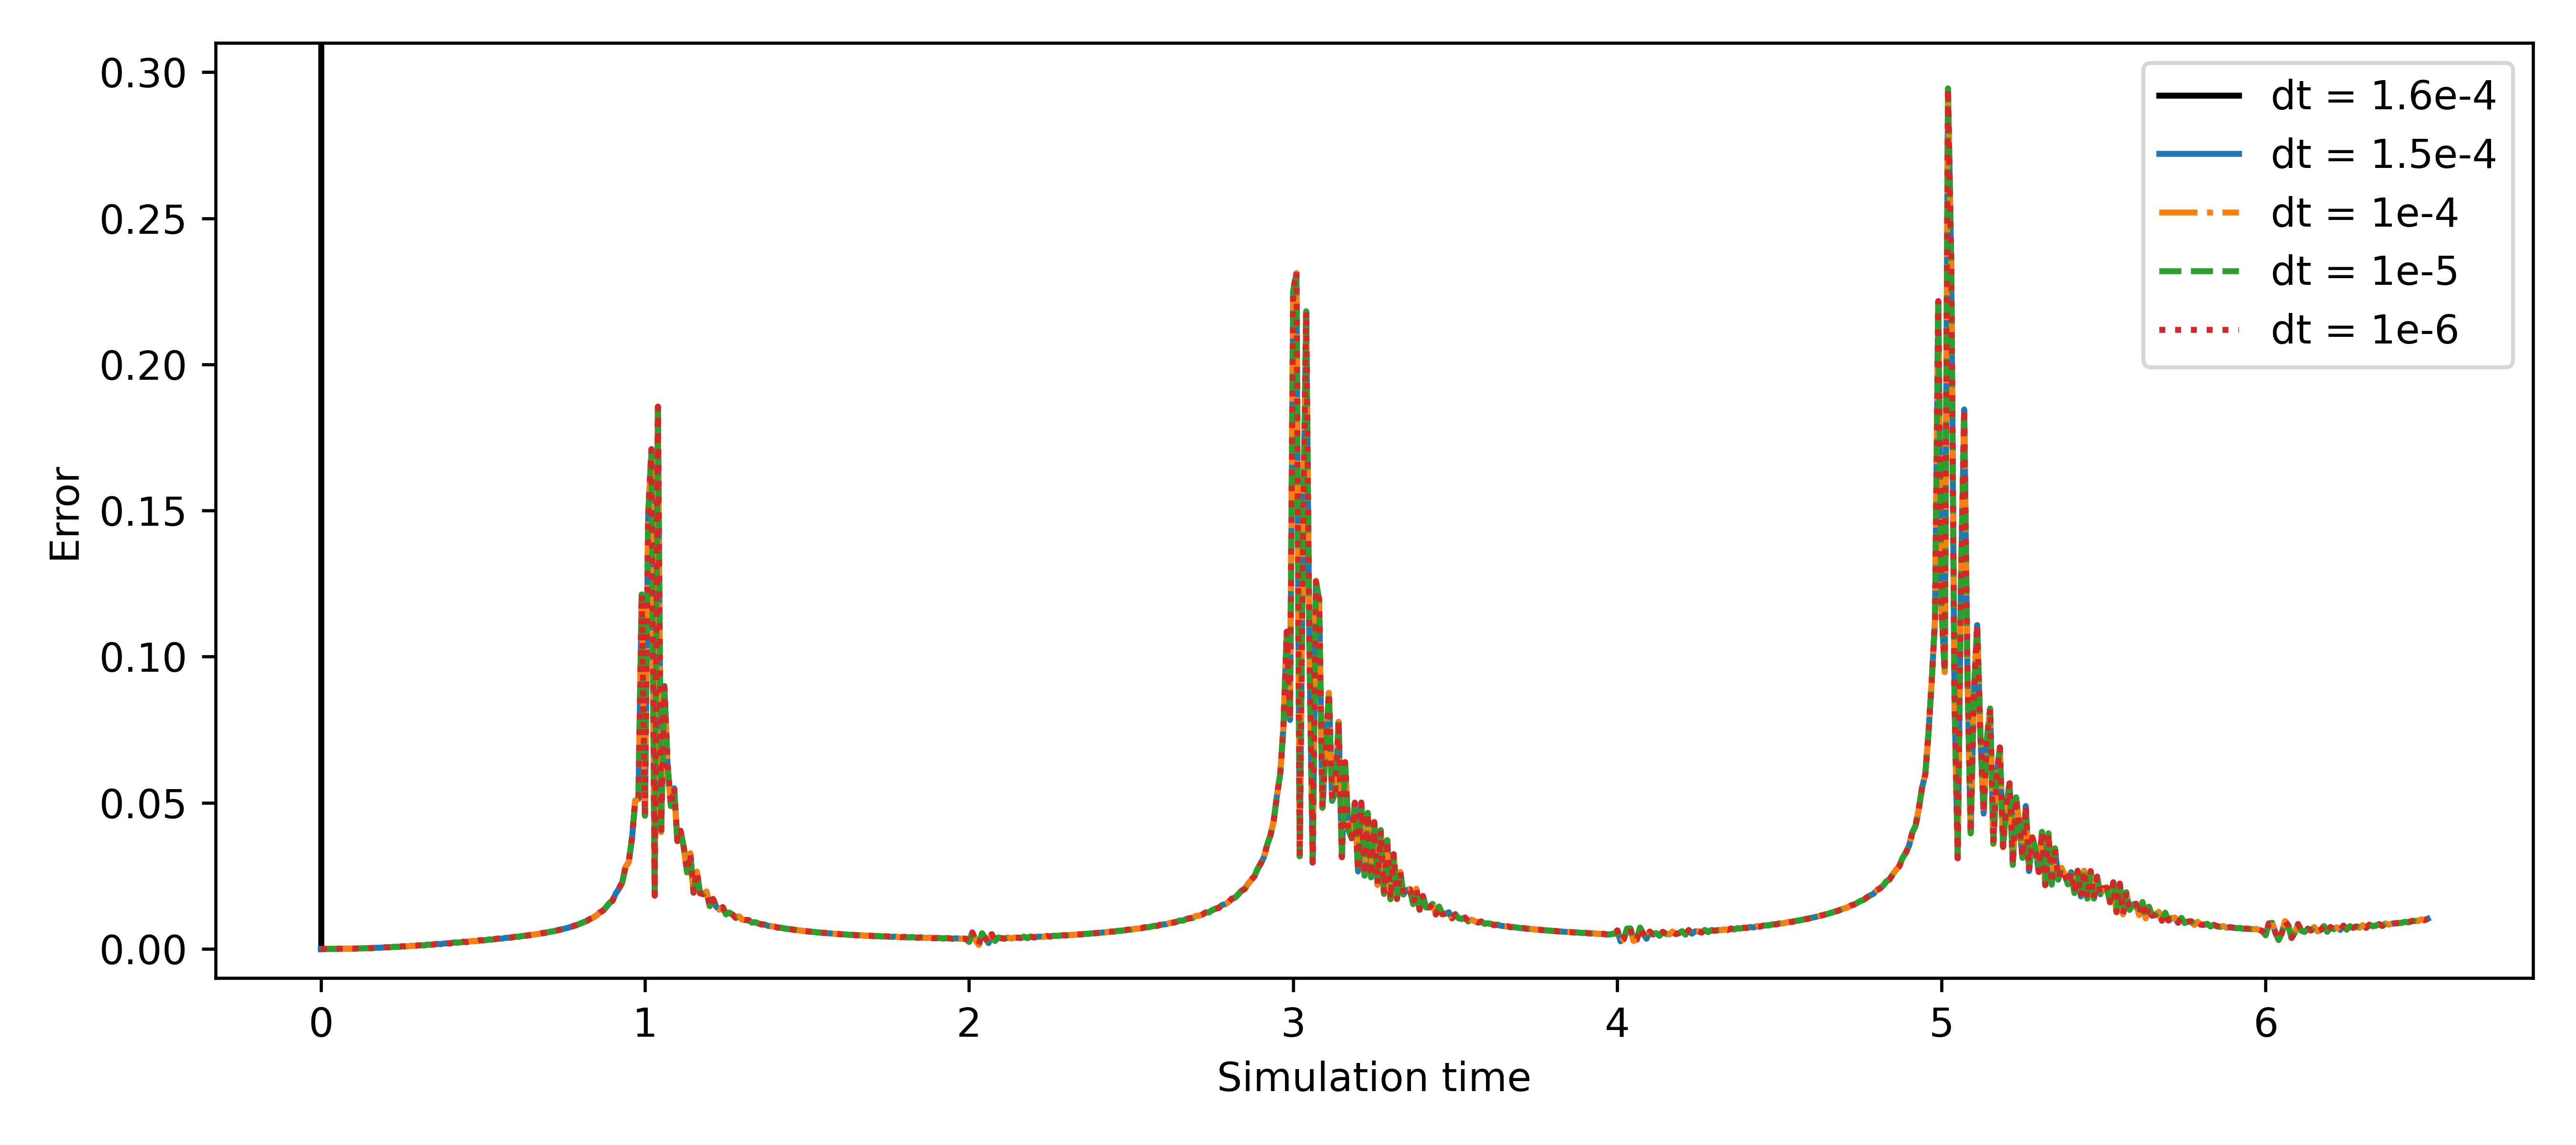
\includegraphics[width = 0.9\textwidth]{media/MSE_comparison.png}
    \caption{Mean square error ($N^{-2} \sum_{i,j} (\phi_\text{anal.}(t) - \phi_\text{num.}(t))^2$ of the simulation ran between $t=0$ and $t=6.5$ for five $\Delta t$ values: $1.6\cdot 10^{-4}, \,1.5\cdot 10^{-4}, \,10^{-4}$,\, $10^{-5}$, and $10^{-6}$.}
\label{MSE_all}\end{figure}
\noindent
The spikes in Figure \ref{MSE_all} correspond to spikes in the plot that occur around odd integer times, as shown in Figure \ref{spikes}. This makes since, since at these times the derivatives of the analytical solution are changing rapidly and so second-order finite difference approximations of them struggle to remain accurate there.
\begin{figure}[H]
    \centering
    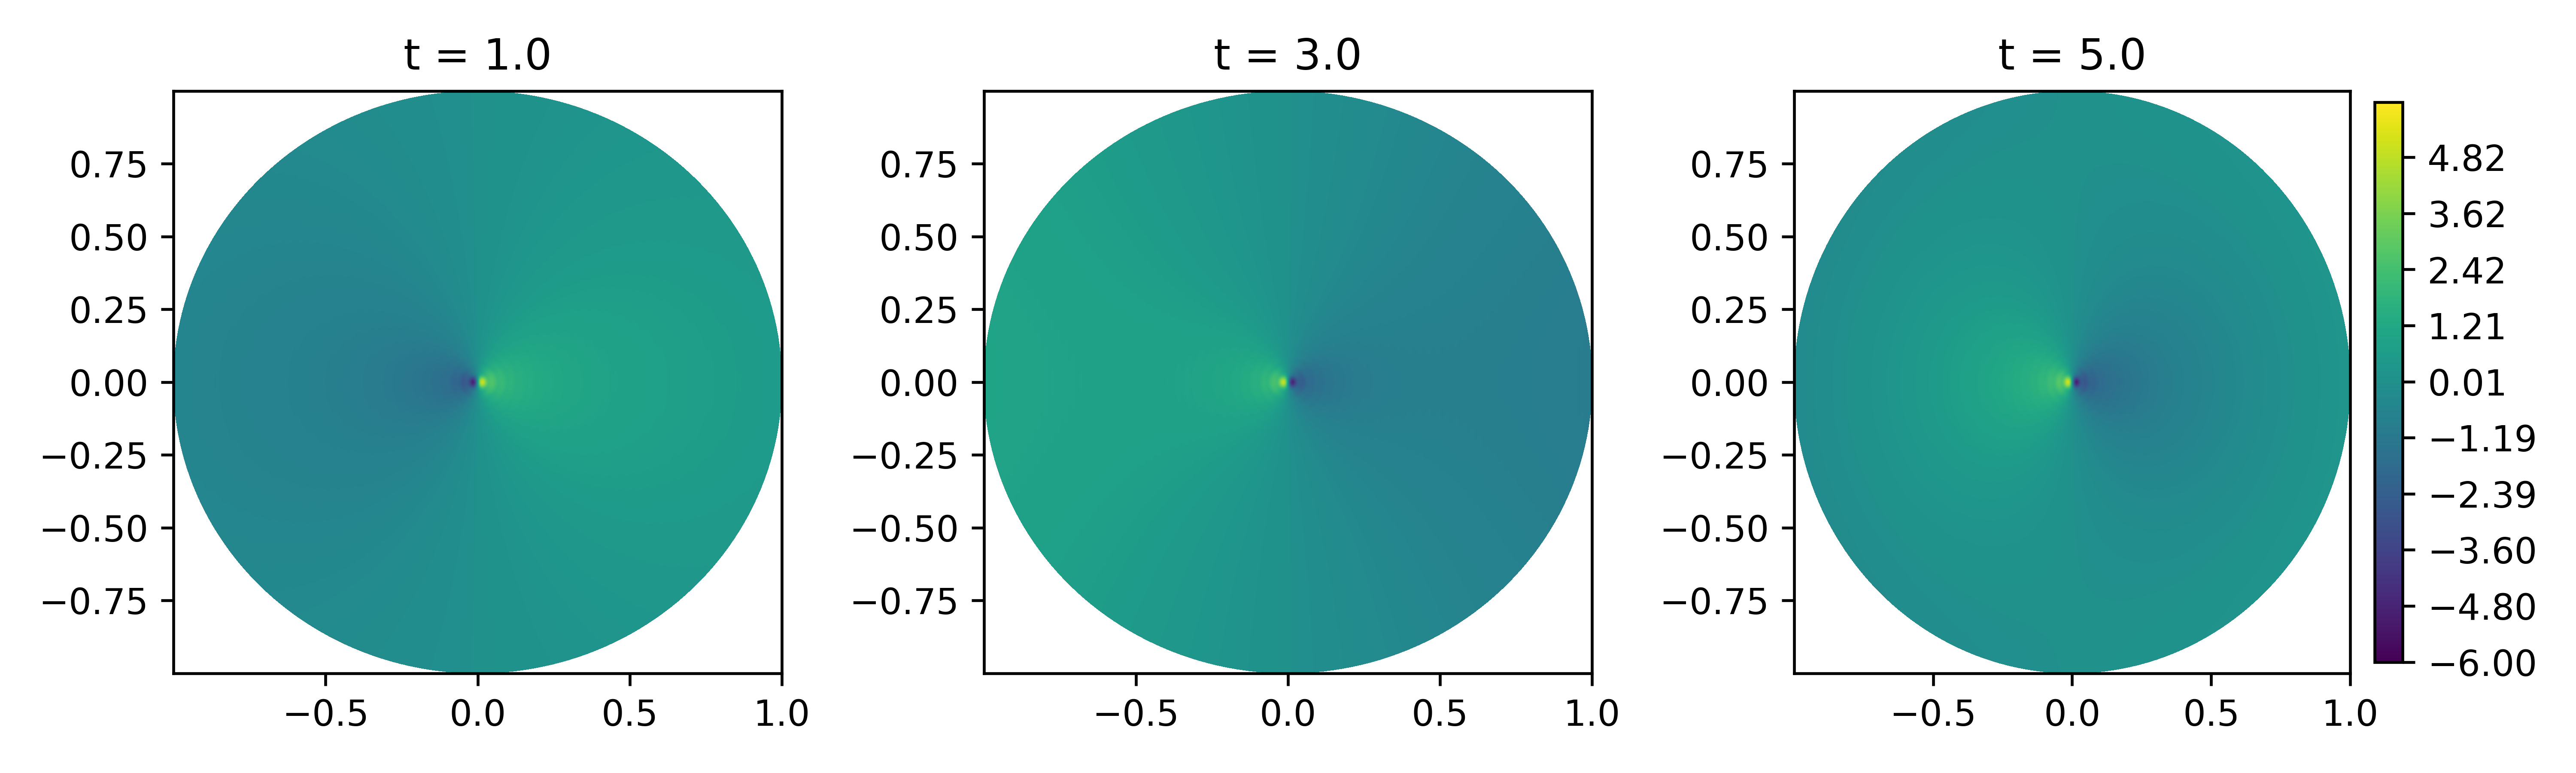
\includegraphics[width = \textwidth]{media/singularities.png}
    \caption{The analytical solution plotted at the times corresponding to the spike in error.}
\label{spikes}\end{figure}
\noindent
The limiting factor in calculating the error over longer runtimes is not the speed of the numerical solution, but that of the analytical solution. This is because at each point and time in the analytical solution, an infinite sum and two integrals must be computed. The analytical solution, however, can be calculated at any time without relying on the knowledge of a previous timestep. Because of this, we also analyzed the difference between the analytical and numerical solutions at times 98, 99, and 100. The MSE at each of these points is, respectively, 0.06, 0.08, and 0.17, which are the same order of magnitude as the MSE for $t\leq 6.5$. Looking back at Figure \ref{big}, is is clear though that the numerical solution gets less accurate as time goes on. The major features are still mostly tracked, but the rippling effect is significantly worse at higher times. Because of this, if the goal were to have the most accurate data in the least amount of time, a mix of analytical and numerical solutions could be used. One could, for example, calculate the expensive analytical solution every ten time units and then run the numerical solution to fill each of the timesteps before the next ten unit time mark. This would limit error buildup.
\\ \\ \noindent
Overall, this method proved highly efficient and highly accurate. It suffered from error buildup as times got larger.

\subsection{Iterative Methods}
After submitting the project proposal, it was discovered that the simple iterative methods that we learned in class are not particularly applicable to this problem. That is because this problem does not easily lend itself to a linear system of the form $\mathbb{A} \mathbf{u} = \mathbf{b}$, where $\mathbf{u}$ is the position data. There are a few reasons for this. The primary one is that there is an isolated second-order time derivative in the governing equation. It it thus quite likely that when the time derivative is discretized using various techniques, $\mathbf{u}_{i,j}^{(n+1)}$ will pop out in a way that is easy to isolate without a matrix inversion. %As such, one would really have to force it to make the problem into a linear system of the type relevant to iterative methods, adding more complication to the solution than is necessary.

\subsection{Time Stepping Methods}
Based on the findings outlined in Section 3.2, a high instability spike can be expected at $t = 1$. Therefore, the following two methods were run to $t = 0.5$ so as to avoid the onset of instabilities due to the unstable nature of time-stepping schemes.
\newpage  \noindent
Both the forward Euler and second-order Runge-Kutta schemes converged to a solution. Figure \ref{time_step_results} shows a qualitative comparison between the results of the numerical results and the analytical solution.
\noindent
Figure \ref{time_step_error} shows an error comparison between the numerical solutions and the analytical solution. One can clearly see that some stability issues have arisen for both of the methods. Time-stepping methods generally converge quickly, but have poor stability, especially when dealing with stiff equations and periodic conditions (which this equation has both of). This is verified by the fact that one can clearly see that the instability arises in a periodic fashion. These instabilities can be subdued by further discretization of the spatial and temporal elements. However, finding the exact stability conditions for this 3-dimensional problem would take a significant amount of time. This is a needlessly convoluted and inefficient process when one could simply utilize methods better suited for stiff PDEs like some of the other schemes described in this report.
\begin{figure}[H]
    \centering
    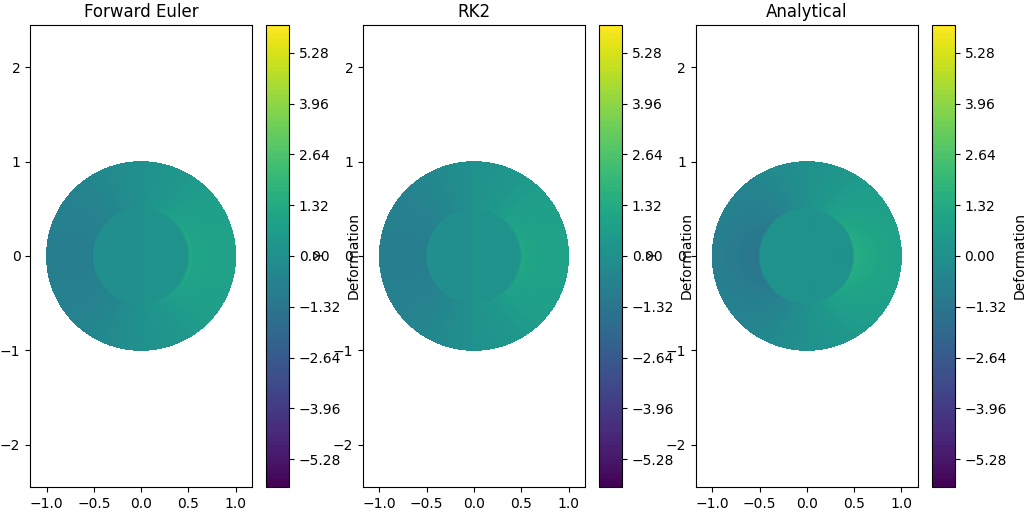
\includegraphics[width = 0.85\textwidth]{media/time_step_compare.png}
    \caption{A comparison of forward Euler, RK2, and the analytical solution at $t=0.5$.}
\label{time_step_results}\end{figure}
\begin{figure}[H]
    \centering
    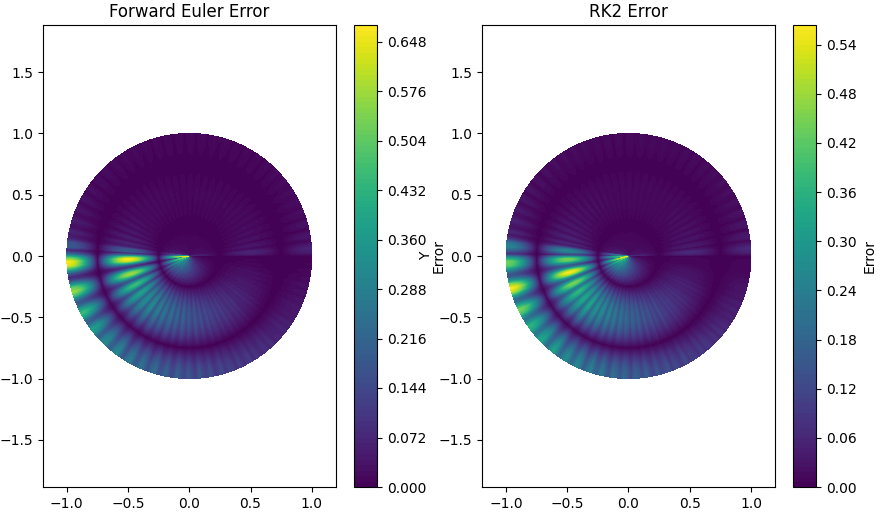
\includegraphics[width = 0.85\textwidth]{media/time_step_error.png}
    \caption{Error of the numerical solutions at $t=0.5$.}
\label{time_step_error}\end{figure}

\subsection{Fourier Spectral Methods}
 The Fourier transform pair of the Laplacian is given:
$$ \frac{{\partial^2 \phi}}{{\partial t^2}} = c^2 \left[ \frac{1}{r} \frac{\partial}{\partial r} \left(r \frac{\partial \phi}{\partial r}\right) + \frac{1}{r^2} \frac{\partial^2 \phi}{\partial \theta^2} \right] \quad \longleftrightarrow \quad \frac{{\partial^2 \hat{\phi}}}{{\partial t^2}} = -c^2 \left( {k_r}^2 \hat{\phi} + \frac{{k_{\theta}}^2}{r^2} \hat{\phi} \right) .$$
\noindent
The time forcing term $\partial^2 \hat{\phi} / \partial t^2$ was progressed using the forward Euler scheme. The solution was then transformed back to the time domain with the inverse $\mathcal{F}^{-1}(\hat{\phi}) = \phi$. The discrete Fast Fourier Transform (FFT) was computed using the \texttt{SciPy} package in \texttt{Python}. First $k_r$ and $k_\theta$ sample frequencies were computed from the $r_i$, $\theta_j$ discretization using \texttt{fftfreq}. Then the transformed Laplacian was computed algebraically and $\hat{\phi}^{(n)}$ was updated according to forward Euler, then transformed into the spatial domain with \texttt{ifft}.
\\ \\ \noindent
This approach was compared with other Fourier algorithms using the \href{https://www.fftw.org/benchfft/}{\texttt{benchFFT}} software program \cite{FFTW05}, on the Princeton \texttt{TIGER} computing cluster. \texttt{TIGER} is a CPU-only HPE \texttt{Linux} cluster on 408 2.4 GHz Skylake nodes (40 cores per node). The Intel C/C++ Compiler 9.0 (flags: \texttt{icc -O3 -xW}) were used. Figure~\ref{fig:Fourier} shows the performance of the \texttt{SciPy} (``FFT\_pack'') Fourier transform package, against \texttt{FFTW 3.1} and \texttt{JMFFTC}. \texttt{JMFFTC} is used by \texttt{NumPy} package, but is optimized for a different architecture (CRAY SCILIB). \texttt{FFTW 3.1} is highly optimized for the \texttt{TIGER} architecture. ``FFTW3\_R2R'' computes discrete transforms using a half-complex transform interface. ``FFTW3\_in\_place'' uses unpacked complex format for real transforms.
\\ \\ \noindent
Speed was measured in floating point operations per second. Error was defined according to the relative L2 Frobenius Norm from the error between the numerical solution and the analytical solution ($\phi^*$)
$$||e||_{L^2} = \sqrt{\frac{1}{N} \sum_{1 \leq i,j \leq N} [\phi \, (r_i, \theta_j) - \phi^*(r_i, \theta_j)]^2}$$
\noindent
The Fourier transform and inverse Fourier transform have time complexity of $\mathcal{O}(N \log(N))$. More precisely, computing the FFT and its inverse gives $2 \, N \log(N)$. Thus overall on an $N^2$ domain yields $\mathcal{O}(N^2 \log(N))$ complexity, significantly faster than differentiation for large $N$. Thus, Figure~\ref{fig:Fourier} shows a scaling $\mathcal{O}(\log(N))$ when plotted against the total grid size (thereby excluding the complexity of looping over the grid) for 1-D transforms of real data up to double-precision. It can be seen that for large $N$ (beyond $N = 2^{14}$) the performance suffers due to memory allocation $\mathcal{O}(\log(N) \, / \, N)$. Further it can be seen that there are significant increases in error for discretizations that are not positive integer powers of 2.

\subsection{\textbf{Performance Engineering}} The accuracy of this numerical simulation is determined largely by the spatial resolution requirements---the solution domain must be large enough to contain the energy-containing motions, and the grid spacing must be small enough to resolve the dissipative scales. The timestep and numerical stability was therefore limited by this discretization and the speed of sound. Performance was optimized by limiting the number of looping functions and using vectorization wherever possible. In the case where looping over the computational grid could not be avoided (and \texttt{NumPy} vectorization was too difficult), the \texttt{Numba} just-in-time compiler was used in ``no Python mode''. With the addition of these features, the code was significantly accelerated and much larger calculations could be achieved.
\newpage
\begin{figure}[H]
    \centering
    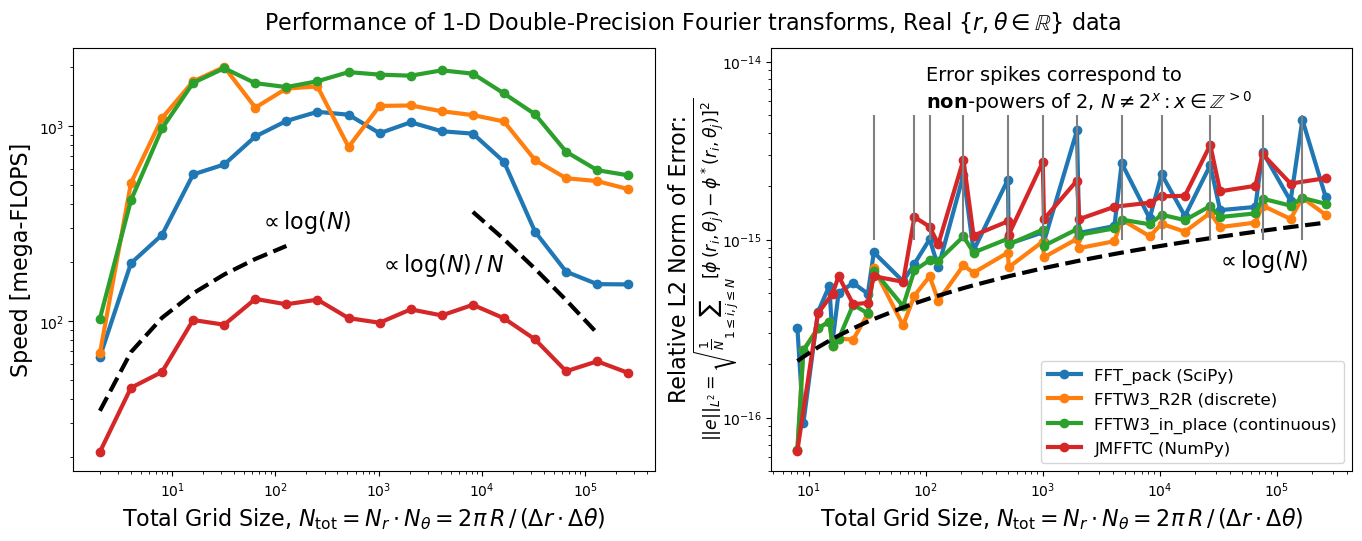
\includegraphics[width = 1.02\textwidth]{media/FFT_performance.png}
    \caption{Benchmark results for the Fourier spectral method solution using the \texttt{benchFFT} program on the Princeton \texttt{TIGER} cluster. It can be seen that for 1-D double-precision transforms of real data, the program scales in speed and relative error $\mathcal{O}(\log(N))$.}
\label{fig:Fourier}\end{figure}

\section{\textbf{Conclusion}}

\subsection{\textbf{Future Work}} The are significant opportunities for improvements to the solvers in speed, stability, and accuracy. Speed could be achieved with spatially varying timesteps or residual averaging. These would all likely degrade accuracy to some degree. Stability can be improved by using higher-order terms of the expansions, such as the inclusion of a second-order term in the time derivative. Accuracy could be improved with techniques that limit the need for artificial smoothing, like using higher-order smoothing, higher-order differencing, or differed corrections. 

Now that the various numerical methods have been evaluated, this approach can be coupled to the $G$-equation, as discussed in the introduction, to provide a deterministic description of flame iso-surface perturbations in turbulent flows. The next steps for this software are to implement parallelization using protocols like \texttt{OpenMP} and \texttt{MPI}.
Methods for more efficient mesh discretization (such as adaptive mesh refinement) were beyond the scope of this project, but could also be implemented to improve accuracy, particularly in the supersonic case.

\subsection{\textbf{Personal Benefits and Lessons Learned}} 
\noindent This project allowed us to develop further proficiency in multiple aspects of the numerical method topics of this course. We work in a computational group (the Computational Turbulent Reacting Flow Laboratory, \href{https://ctrfl.princeton.edu/}{CTRFL}) and this course genuinely helped us understand the numerical methods implemented in our existing solvers, like \href{https://github.com/desjardi/NGA2}{NGA}, \href{https://ctrfl.princeton.edu/software/}{PDRs}, \href{https://computing.llnl.gov/projects/sundials}{SUNDIALS}, \href{https://computing.llnl.gov/projects/hypre-scalable-linear-solvers-multigrid-methods}{HYPRE}, \href{https://www.netlib.org/lapack/}{LAPACK}, and \href{https://www.fftw.org/}{FFTW}, giving us more exposure to its syntax and code format that will be greatly useful to us in our future research. While not relevant to this project, the course content in massively parallel architectures was also extremely relevant to our research.

We learned that while \texttt{Git} is an essential tool for collaboration and version control, real-world communication is essential. Further, one must be deliberate in changes that are made, including writing code in a ``linear'' way when possible, such that merge conflicts are straightforward to resolve. However, the software development process itself cannot be linear, one must engage in test- and performance-driven development, designing with these aspects in mind from the start.

\subsection{\textbf{Software Repository}} This report presents the development of \href{https://github.com/mw6136/WAVE}{\texttt{WAVE}}, a software repository for comparing numerical methods on cylindrical wave equation solver performance. The repository consists of the various solvers, with a data output and visualization scheme. The analytical solution has also been visualized for comparison. More figures and visualizations are available in the repository on \texttt{Github}. Further instructions on running the program are available in the \texttt{README}. The report and presentation submission documents are also available on the repository.

\bibliographystyle{plain}
\bibliography{citations}

\newpage
\appendix
\section{Wave Equation Classification and 1-D Solution} \label{A}
\subsection{Wave Equation Classification}
The wave equation is a second-order linear partial differential equation (PDE) for the description of waves or standing wave fields. The scalar wave equation describes the mechanical wave propagation of any scalar $\phi$ as 
\[ \frac{\partial^2 \phi}{\partial t^2} = c^2 \left(\frac{\partial^2 \phi}{\partial x^2} + \frac{\partial^2 \phi}{\partial y^2} + \frac{\partial^2 \phi}{\partial z^2}  \right) = c^2 \,\nabla^2 \, \phi \quad ,\]
\noindent
where $c$ is a fixed non-negative real coefficient. $\nabla$ is the \emph{nabla} operator and $\nabla^2 = \nabla \cdot \nabla \equiv \frac{\partial^2}{\partial x^2} + \frac{\partial^2}{\partial y^2} + \frac{\partial^2}{\partial z^2}$ is the spatial Laplacian operator (in Cartesian coordinates). Because the wave equation is linear and homogeneous, it can be analyzed as a linear combination (superposition) of simple solutions that are sinusoidal plane waves with various directions of propagation and wavelengths, but all with the same finite propagation speed $c$. 
\\[5pt] \noindent
Projecting the wave equation in the general form of a second-order PDE

\[ A \frac{\partial^2 \phi}{\partial t^2} + B \frac{\partial^2 \phi}{\partial x \partial t} + C \frac{\partial^2 \phi}{\partial x^2} + D \frac{\partial \phi}{\partial t} + E \frac{\partial \phi}{\partial x} + F \phi = 0 \]
\\ \noindent
gives $A = 1$, $B = 0$, and $C = -c^2$, and thus the discriminant $B^2 - 4AC > 0$ defines a hyperbolic PDE with a well-posed initial value problem.

\subsection{Algebraic Solution to the 1-D Wave Equation}
A solution to the wave equation in 1-D is rather trivial and demonstrates that any solution can be formed as a linear combination of \emph{standing waves}. The wave equation in one spatial dimension
\[ \frac{\partial^2 \phi}{\partial t^2} = c^2 \, \frac{\partial^2 \phi}{\partial x^2} \]
\noindent
is unusual for a partial differential equation in that a relatively simple general solution may be found. Using an algebraic change of variable $\xi = x - ct$ and  $\eta = x + ct$, and computing the partial derivatives
\begin{align*}
\frac{\partial \phi}{\partial t} &= \frac{\partial \phi}{\partial \xi} \frac{\partial \xi}{\partial t} + \frac{\partial \phi}{\partial \eta} \frac{\partial \eta}{\partial t}
\\
\frac{\partial^2 \phi}{\partial t^2} &= c^2 \frac{\partial^2 \phi}{\partial \xi^2} -2c \frac{\partial^2 \phi}{\partial \xi \partial \eta} + c^2 \frac{\partial^2 \phi}{\partial \eta^2}
\\[8pt]
\frac{\partial \phi}{\partial x} &= \frac{\partial \phi}{\partial \xi} + \frac{\partial \phi}{\partial \eta}
\\
\frac{\partial^2 \phi}{\partial x^2} &= \frac{\partial^2 \phi}{\partial \xi^2} + 2 \frac{\partial^2 \phi}{\partial \xi \partial \eta} + \frac{\partial^2 \phi}{\partial \eta^2} \quad .
\end{align*}
\noindent
Substituting into the wave equation for $c \neq 0$, the wave equation becomes
\[ \frac{\partial^2 \phi}{\partial \xi \partial \eta }(x,t) = 0 \quad ,\]
which is separable and can be integrated for a general solution, where $F$, $G$, $H$ are arbitrary forcing functions.
\[ \int \frac{\partial^2 \phi}{\partial \xi \partial \eta } \, d \xi = 0 \rightarrow \frac{\partial \phi}{\partial \eta} = H(\eta) \]
\[ \phi(\xi, \eta) = \int \frac{\partial \phi}{\partial \eta} \, d \eta = \int H(\eta) \, d \eta + F(\xi) = F(\xi ) + G(\eta ) \]

\[ \phi(x, t) = F(x - ct) + G(x - ct) \quad .\]
\\ \noindent
Thus the solutions of the 1-D wave equation are sums of a right-translating function $F$ and a left-translating function $G$ at the speed $c$.
\newpage
\section{Analytical Solution to the Wave Equation in Cylindrical Coordinates} \label{B}

\subsection{The Wave Equation in Cylindrical Coordinates}
For circularly propagating waves, it is useful to project the wave equation in cylindrical coordinates.

\[ \frac{\partial^2 \phi}{\partial t^2} = c^2 \left(\frac{\partial^2 \phi}{\partial x^2} + \frac{\partial^2 \phi}{\partial y^2} + \frac{\partial^2 \phi}{\partial z^2}  \right) = c^2 \,\nabla^2 \, \phi \]
\\ \noindent
Substituting the transformation from Cartesian variables $(x, y, z)$ to cylindrical $(r, \theta, z)$, $ x = r \cos{\theta}$, $y = r \sin{\theta}$, and $r^2 = x^2 + y^2$, $\theta =\tan^{-1} (y / x)$. 

\begin{figure}[h]
    \begin{center}
    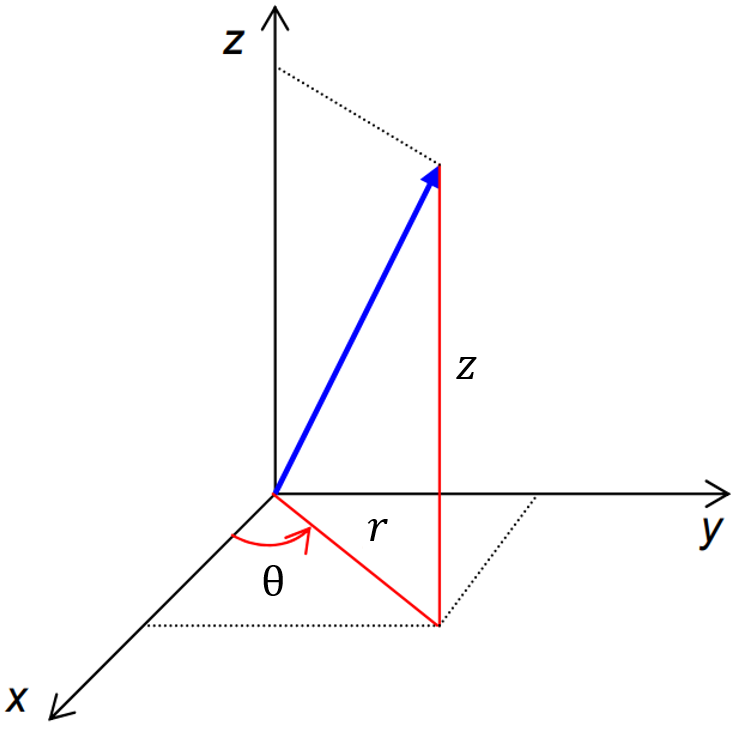
\includegraphics[scale = 0.25]{media/Cylindrical-Coordinates.png}
    \caption{Cartesian and Cylindrical coordinates.}
    \end{center}
\end{figure}
\noindent
The partial derivatives can be evaluated as:
\begin{align*}
\frac{\partial r}{\partial x} &= \frac{x}{r} = \cos(\theta) \qquad \frac{\partial r}{\partial y} = \frac{y}{r} = \sin(\theta) \\
\frac{\partial \theta}{\partial x} &= -\frac{\sin(\theta)}{r} \qquad \quad \; \frac{\partial \theta}{\partial y} = \frac{\cos(\theta)}{r}
\end{align*}
Applying the chain rule:
\begin{align*}
\frac{\partial \phi}{\partial x} = \frac{\partial \phi}{\partial r} \frac{\partial r}{\partial x} + \frac{\partial \phi}{\partial \theta} \frac{\partial \theta}{\partial x}\\
\frac{\partial \phi}{\partial y} = \frac{\partial \phi}{\partial r} \frac{\partial r}{\partial y} + \frac{\partial \phi}{\partial \theta} \frac{\partial \theta}{\partial y}
\end{align*}
Therefore, the Laplacian in cylindrical coordinates is
\[ \nabla^2 \;\; = \;\; \frac{\partial^2}{\partial x^2} + \frac{\partial^2}{\partial y^2} + \frac{\partial^2}{\partial z^2} \;\; = \;\; \frac{\partial^2}{\partial r^2} + \frac{1}{r} \frac{\partial}{\partial r} + \frac{1}{r^2} \frac{\partial^2}{\partial \theta^2} + \frac{\partial^2}{\partial z^2} \]
\noindent
and the wave equation can be written as

\[ \frac{1}{c^2} \frac{\partial^2 \phi }{\partial t^2 } = \frac{\partial^2 \phi }{\partial r^2 } + \frac{1}{r} \frac{\partial \phi }{\partial r} + \frac{1}{r^2 } \frac{\partial^2 \phi }{\partial \theta^2 } + \cancel{\frac{\partial^2 \phi }{\partial z^2 }} \quad .\]
\\ \noindent
It is clear that it remains a hyperbolic PDE, but now with a singular point at the origin $r = 0$. The study of surface deformation requires only plane-polar coordinates, so the $\partial^2 \phi / \partial z^2$ term may be neglected. We now seek an analytical solution to the 2-D equation, given well-posed boundary and initial conditions.
\newpage
\subsection{\textbf{Problem Statement}}
\noindent Note: this problem was adapted from Problem Set 9, Exercise 3 of Princeton University Course MAE501: Mathematical Methods of Engineering Analysis I in Fall semester 2023 \cite{MAE501}.
\\ \\
\noindent For a small deformation of any planar circular elastic material, the surface deformation, $\phi$, satisfies the wave equation in plane-polar coordinates

\[ \frac{\partial^2 \phi}{\partial t^2} = c^2 \left[ \frac{1}{r} \frac{\partial}{\partial r} \left(r \frac{\partial \phi}{\partial r}\right) + \frac{1}{r^2} \frac{\partial^2 \phi}{\partial \theta^2} \right]\]
\\
\noindent where the driving force of the wave motion for a material initially at rest can be specified through the boundary and initial conditions. Seeking to model waves on the surface of the fluid generated by the motion of the walls, we choose the following boundary and initial conditions. \\[8pt]
\noindent Boundary Conditions: \\
$ \phi(r=R, \theta, t) = A \cos(\omega t) \cos (\theta) $ \\
$ \phi(r=0, \theta, t) \rightarrow \textrm{finite} $ \\
$ \phi(r, \theta + 2\pi, t) = \phi(r, \theta, t) $ \\[8pt]
\noindent Initial Conditions: \\
$ \phi(r, \theta, t=0) = 0 $ \\
$ \partial \phi/ \partial t \, (r, \theta, t=0) = 0 $

\subsection{Method of Solution}
We will solve for $\phi$ for all $t$, $\theta$, and $r$ using the method of separation of variables and eigenfunction expansions. We will also determine the resonance condition for the value of $\omega$. 
\\[8pt]
\noindent Steps in the solution:
\begin{enumerate}
    \item Use Separation of Variables to de-couple the time component and determine the eigenfunctions for the operator with boundary conditions
    \[ \nabla^2 \psi = \left[ \frac{1}{r} \frac{\partial}{\partial r} \left(r \frac{\partial \psi}{\partial r}\right) + \frac{1}{r^2} \frac{\partial^2 \psi}{\partial \theta^2} \right] = - \lambda \psi \]
    \noindent Boundary Conditions: \\
    $ \psi(r=R, \theta) = 0 $ \\
    $ \psi(r=0, \theta) \rightarrow \textrm{finite} $ \\
    $ \psi(r, \theta + 2\pi) = \psi(r, \theta) $ \\
    \item Determine a function $\tilde{\phi}$, that when subtracted from $\phi$ makes the boundary conditions homogeneous but perhaps introduces inhomogeneities in the initial conditions and the equation itself.
    \item Use the eigenfunctions determined from the separation of variables in the method of eigenfunction expansions and solve for $\phi$.
\end{enumerate} 
\newpage
\subsection{Final Solution}
\noindent These conditions lead to the analytical solution 
$$ \phi(r, \theta, t) = A \left(\frac{r}{R} \right)^2 \cos(\omega t) \cos(\theta) + \tilde{\phi} (r, \theta, t)$$ 

\noindent $\tilde{\phi}$ is composed as follows, where $J_n (\cdot)$ is the Bessel function of the 1st kind and order $n$, $\eta$ is a variable of integration, and $\lambda$ are the eigenfunctions for each of the modes.
$$ \tilde{\phi} (r, \theta, t) = \sum_{m=1}^\infty \Biggl( \frac{1}{c^2 \lambda_{n,m} - \omega^2} \frac{2A}{R^2} \frac{\int_0^1 \left( \omega^2 \eta^2 + 3c^2 \right) \eta J_1\left( \sqrt{\lambda_{1,m}} R \eta \right) d\eta }{{J_2}^2 \left( \sqrt{\lambda_{1,m}} R \right)} \cos(\omega t) \; \dots $$

$$ - \frac{2A}{{J_2}^2 \left( \sqrt{\lambda_{1,m}} R \right)}\Bigg[ \int_0^1 \eta^3 J_1 \left( \sqrt{\lambda_{1,m}} R\eta \right) d\eta \; \dots $$

$$ + \frac{1}{c^2 \lambda_{n,m} - \omega^2} \frac{1}{R^2} \int_0^1 \left(\omega^2 \eta^2 + 3c^2 \right) \eta J_1 \left(\sqrt{\lambda_{1,m}} R \eta \right) d\eta \Bigg] \cos \left(c \sqrt{\lambda_{1,m}} t \right) \Biggl) \cos(\theta) J_1 \left(\sqrt{\lambda_{1,m} } r \right) .$$

\subsection{Full Derivation}
\noindent The method of Separation of Variables can be applied to a partial differential equation (PDE) when the equation is linear and homogeneous, where the boundary conditions are also linear and homogeneous. Thus, considering the homogeneous stationary boundary value problem, using separation of variables, assume $\phi(r, \theta, t) = \psi (r, \theta) \mathcal{T} (t)$ and substituting in the wave equation

\[ \frac{\partial^2 (\psi \mathcal{T})}{\partial t^2} = c^2 \left[ \frac{1}{r} \frac{\partial}{\partial r} \left(r \frac{\partial (\psi \mathcal{T})}{\partial r}\right) + \frac{1}{r^2} \frac{\partial^2 (\psi \mathcal{T})}{\partial \theta^2} \right] \quad \rightarrow \quad \psi \mathcal{T}'' = c^2 \left[ \frac{\mathcal{T}}{r} \frac{\partial}{\partial r} \left(r \frac{\partial \psi}{\partial r}\right) + \frac{\mathcal{T}}{r^2} \frac{\partial^2 \psi}{\partial \theta^2} \right] \quad .\]
\\ \noindent
Dividing by $\psi \mathcal{T} c^2$,
\[ \frac{1}{\psi} \left[ \frac{1}{r} \frac{\partial}{\partial r} \left(r \frac{\partial \psi}{\partial r}\right) + \frac{1}{r^2} \frac{\partial^2 \psi}{\partial \theta^2} \right] = \frac{1}{c^2} \frac{\mathcal{T}''}{\mathcal{T}} = - \lambda \quad ,\]
\\ \noindent
with $\lambda$ a constant that will be shown to correspond to the eigenfunctions for each of the modes. Now using separation of variables again on the spatial component, assume $ \psi (r, \theta) = \mathcal{R}(r) \, \Theta(\theta) $ and again substitute into the $\nabla^2 \psi$ operator

\[ \frac{1}{r} \frac{\partial}{\partial r} \left(r \frac{\partial (\mathcal{R} \Theta)}{\partial r}\right) + \frac{1}{r^2} \frac{\partial^2 (\mathcal{R} \Theta)}{\partial \theta^2} = - \lambda \mathcal{R} \Theta \quad \rightarrow \quad \frac{\Theta}{r} (\mathcal{R}' + r \mathcal{R}'') + \frac{\mathcal{R} \Theta''}{r^2} = - \lambda \mathcal{R} \Theta \quad .\]
\noindent
The PDE can then be rewritten as
\[ \frac{1}{\mathcal{R}} r \frac{d}{dr} \big(r \mathcal{R'} \big) + \lambda r^2 = -\frac{\Theta''}{\Theta}  = \alpha^2 \]
\\ \noindent
with $\alpha^2$ as some constant. First solving the angular component by applying an integrating factor and solving for the roots of the characteristic polynomial $\Theta \sim \exp(\delta \theta) \rightarrow \delta = \pm \alpha i$, then substituting Euler's identity $\exp(i \alpha) = \cos(\alpha) + i \, \sin(\alpha)$. 

\[ \Theta'' = -\alpha^2 \Theta \quad \rightarrow \quad \Theta (\theta) = a \cos(\alpha \theta) + b \sin(\alpha \theta) \quad .\]
\noindent
Applying the condition $\psi(r, \theta + 2\pi) = \psi(r, \theta)$,
\begin{equation*}
    \begin{split}
        a &\cos(\alpha \theta + \alpha 2 \pi) + b \sin(\alpha \theta + \alpha 2 \pi) = a \cos(\alpha \theta) + b \sin(\alpha \theta) \\
        &\rightarrow  \cos(\alpha \theta + \alpha 2 \pi) = \cos(\alpha \theta) \quad \textrm{and} \quad \sin(\alpha \theta + \alpha 2 \pi) = \sin(\alpha \theta) \\
        &\rightarrow \alpha_n = n \in \mathbb{Z}^{\geq 0} \;\; \textrm{an integer}
    \end{split}
\end{equation*}

\noindent
Therefore a solution to the angular problem is
\[\Theta_n (\theta) = a_n \cos(n \theta) + b_n \sin(n \theta) \quad . \]
\noindent
Now re-arranging the radial problem (where the substitution $\alpha_n = n$) is made,
\[ \frac{1}{\mathcal{R}} r \frac{d}{dr} \big(r \mathcal{R'} \big) + \lambda r^2 = n^2 \quad \rightarrow \quad r \frac{d}{dr} \big(r \mathcal{R'} \big) + (\lambda r^2 - n^2) \mathcal{R} = 0 \]
\[ r^2 \mathcal{R}'' + r \mathcal{R}' + (\lambda r^2 - n^2) \mathcal{R} = 0 \]
\noindent 
This is the form of a Bessel equation of order $n$ and therefore the solutions to the radial problem are the Bessel functions of order $n$,
\[\mathcal{R}(r) = c J_n (\sqrt{\lambda} r) + d \cancel{Y_n (\sqrt{\lambda} r)} \quad .\]

\noindent
Applying boundary conditions: \\
\noindent $\mathcal{R}(r = 0) \; \textrm{finite} \; \rightarrow \; d = 0$ \\
\noindent $\mathcal{R}(r = R) = 0 \; \rightarrow \; c J_n (\sqrt{\lambda_{n,m}} r) = 0 \; \rightarrow \; \sqrt{\lambda_{n,m}} r = z_{n,m} \; \textrm{for} \; c \neq 0$ \\ \\ \noindent
This gives a relation between the eigenvalues and zeroes of the Bessel function,  where $z_{n,m}$ is the $m$-th zero of the $n$-th order Bessel function $J_n$ for $m = 1,2,3 \dots$ Therefore the eigenfunctions  are of the form 
\[ \psi_{n,m} (r, \theta) = \mathcal{R}(r) \, \Theta(\theta) = [a_{n,m} \cos(n \theta) + b_{n,m} \sin(n \theta)] J_n (\sqrt{\lambda_{n,m}} r) \]
\\ \noindent
With the modes of $a_{n,m}(t)$ and $b_{n,m}(t)$ to be determined as functions of time. Now considering the original problem, the boundary condition is inhomogeneous, so we must rescale the problem to achieve homogeneous boundary conditions. Let
\[ \tilde{\phi} \equiv \phi - A \left(\frac{r}{R} \right)^2 \cos(\omega t) \cos(\theta) \]
\noindent
Here the $r^2 / R^2$ term is necessary to resolve the singularity from the ODE. Taking the time and spatial derivatives of $\tilde{\phi}$ to rewrite the PDE:
\begin{align*}
\frac{ \partial \phi}{\partial t} &= \frac{ \partial \tilde{\phi}}{\partial t} - A \omega \left(\frac{r}{R} \right)^2 \sin(\omega t) \cos(\theta) \\
\frac{ \partial \phi}{\partial r} &= \frac{ \partial \tilde{\phi}}{\partial r} - 2 A \left(\frac{r}{R^2}\right) \cos(\omega t) \cos(\theta) \\
\frac{ \partial^2 \phi}{\partial t^2} &= \frac{ \partial^2 \tilde{\phi}}{\partial t^2} - A \omega^2 \left(\frac{r}{R} \right)^2 \cos(\omega t) \cos(\theta) \\
\frac{1}{r} \frac{\partial}{\partial r} (r \frac{\partial \phi}{\partial r}) &= \frac{1}{r} \frac{\partial}{\partial r} (r \frac{\partial \tilde{\phi}}{\partial r}) + 4 A \left(\frac{1}{R^2}\right) \cos(\omega t) \cos(\theta) \\
\frac{1}{r^2} \frac{\partial^2 \phi }{\partial \theta^2} &= \frac{1}{r^2} \frac{\partial^2 \tilde{\phi} }{\partial \theta^2} - A \left(\frac{1}{R^2}\right) \cos(\omega t) \cos(\theta)
\end{align*}
\noindent
Now combining to rewrite the solution in terms of the transformed variable $\tilde{\phi}$,
\[ \frac{ \partial^2 \tilde{\phi}}{\partial t^2} - A \omega^2 \left(\frac{r}{R} \right)^2 \cos(\omega t) \cos(\theta) = c^2 \left[ \frac{1}{r} \frac{\partial}{\partial r} (r \frac{\partial \tilde{\phi}}{\partial r}) + \frac{4A}{R^2} \cos(\omega t) \cos(\theta) + \frac{1}{r^2} \frac{\partial^2 \tilde{\phi} }{\partial \theta^2} - \frac{A}{R^2} \cos(\omega t) \cos(\theta) \right]\]
\noindent
which simplifies as
\[ \frac{ \partial^2 \tilde{\phi}}{\partial t^2} - \frac{A}{R^2} \cos(\omega t) \cos(\theta) (\omega^2 r^2 + 3c^2) = c^2 \left[ \frac{1}{r} \frac{\partial}{\partial r} (r \frac{\partial \tilde{\phi}}{\partial r}) + \frac{1}{r^2} \frac{\partial^2 \tilde{\phi} }{\partial \theta^2} \right] \quad .\]
\noindent The initial and boundary conditions are similarly re-scaled.
\\ [8pt]
\noindent Boundary Conditions: \\
$ \tilde{\phi}(r=R, \theta, t) = 0 $ \\
$ \tilde{\phi}(r=0, \theta, t) \rightarrow \textrm{finite} $ \\
$ \tilde{\phi}(r, \theta + 2\pi, t) = \tilde{\phi}(r, \theta, t) $ \\ [8pt]
\noindent Initial Conditions: \\
$ \tilde{\phi}(r, \theta, t=0) = - A \left( \frac{r^2}{R^2} \right) \cos(\theta) $ \\
$ \partial \tilde{\phi}/ \partial t \, (r, \theta, t=0) = 0 $ \\ [8pt] \noindent
Note that the boundary conditions are now homogeneous, but one of the initial conditions is inhomogeneous. For convenience, define a function
\[ f(r, \theta , t) \equiv A \left( \frac{1}{R^2} \cos(\omega t) \cos(\theta) (\omega^2 r^2 + 3c^2) \right) \quad .\]
\noindent
Solving the new PDE in $\tilde{\phi}$ we expand the inhomogeneity $f(r, \theta , t)$ in the eigenfunctions of the stationary problem
\[ f(r, \theta , t) = \sum^\infty_{n=0} \sum^\infty_{m=0} [c_{n,m}(t) \cos(n \theta) + d_{n,m}(t) \sin(n \theta) ] J_n (\sqrt{\lambda_{n,m}} r) \]
\noindent
Using orthogonality of eigenfunctions we can solve for $c_{n,m}(t)$ and $d_{n,m}(t)$ by calculating the inner product using an appropriate weight function $r$

\[ c_{n,m}(t) = \frac{\langle f(r, \theta, t), J_n (\sqrt{\lambda_{n,m}} r) \cos(n \theta) \rangle_r}{\langle J_n (\sqrt{\lambda_{n,m}} r) \cos(n \theta), J_n (\sqrt{\lambda_{n,m}} r) \cos(n \theta) \rangle_r} = \frac{\int^R_0 \int^{2 \pi}_0 f(r, \theta , t) r J_n (\sqrt{\lambda_{n,m}} r) \cos(n \theta) dr \, d \theta}{\int^R_0 \int^{2 \pi}_0 r {J_n}^2 (\sqrt{\lambda_{n,m}} r) \cos^2(n \theta) dr \, d \theta} \]
\[ d_{n,m}(t) = \frac{\langle f(r, \theta, t), J_n (\sqrt{\lambda_{n,m}} r) \sin(n \theta) \rangle_r}{\langle J_n (\sqrt{\lambda_{n,m}} r) \sin(n \theta), J_n (\sqrt{\lambda_{n,m}} r) \sin(n \theta) \rangle_r} = \frac{\int^R_0 \int^{2 \pi}_0 f(r, \theta , t) r J_n (\sqrt{\lambda_{n,m}} r) \sin(n \theta) dr \, d \theta}{\int^R_0 \int^{2 \pi}_0 r {J_n}^2 (\sqrt{\lambda_{n,m}} r) \sin^2(n \theta) dr \, d \theta} \]
\noindent
We can rewrite 
\begin{multline*}
\int^R_0 \int^{2 \pi}_0 f(r, \theta , t) \, r J_n (\sqrt{\lambda_{n,m}} r) \cos(n \theta) \, dr \, d \theta \;=\\ \frac{A}{R^2} \cos(\omega t) \left[ \int^{2 \pi}_0 \cos(\theta) \cos(n \theta) \, d \theta \int^R_0 (\omega^2 r^2 + 3c^2)  r J_n (\sqrt{\lambda_{n,m}} r) \, d r \right]
\end{multline*}
\noindent
Because $\cos(n \theta)$ are orthogonal functions, only when $n = 1$ is $c_{n,m}$ non-zero.
\[ \int^{2 \pi}_0 \cos(\theta) \cos(n \theta) d \theta = 
\begin{cases}
      \pi & \text{if $n=1$}\\
      0 & \text{if $n \neq 1$}\\
    \end{cases}
\]
\noindent
Thus $c_{n,m}$ simplifies to 
\[ c_{n,m} = 
\begin{cases}
      0 & \text{if $n \neq 1$}\\
      \frac{2A}{R^4} \cos(\omega t) \frac{\int^R_0 (\omega^2 r^2 + 3c^2)  r J_1 (\sqrt{\lambda_{1,m}} r) \, d r}{{J_2}^2 (\sqrt{\lambda_{1,m}} R) } & \text{if $n = 1$}\\
    \end{cases}
\]
\noindent
This also requires the integration property of Bessel functions $\int x^n J_{n-1}(x) dx = x^n J_n(x)$. Similarly, as $f(r, \theta, t)$ is only a function of cosine, 

\[ \int^{2 \pi}_0 \cos(\theta) \sin(n \theta) d \theta = 0 \,\forall \, n \quad \rightarrow \quad d_{n,m} = 0 \; .\]
\noindent
Since $\cos(\theta)$ corresponds to $m = 1$ and $\cos(n \theta)$ is orthogonal to $\cos(m \theta)$ for $ n \neq m$, all terms $n \neq 1$ are 0 and the summation over $n$ can be removed.

\[ f(r, \theta , t) = \frac{2A}{R^4} \cos(\omega t) \sum^\infty_{m=1} \frac{\int^R_0 (\omega^2 \zeta^2 + 3c^2)  \zeta J_1 (\sqrt{\lambda_{1,m}} \zeta) d \zeta}{{J_2}^2 (\sqrt{\lambda_{1,m}} R) } \cos(\theta) J_1(\sqrt{\lambda_{n,m}} r)\]
\noindent
Here $\zeta$ is the variable of integration. If we non-dimensionalize the variable in the integral with $R \eta = \zeta$,

\[ f(r, \theta , t) = \frac{2A}{R^2} \cos(\omega t) \sum^\infty_{m=1} \frac{\int^1_0 (\omega^2 \eta^2 + 3c^2)  \eta J_1 (\sqrt{\lambda_{1,m}} R \eta) d \eta}{{J_2}^2 (\sqrt{\lambda_{1,m}} R) } \cos(\theta) J_1(\sqrt{\lambda_{n,m}} r) \quad .\]
\\ \noindent
Similar to the stationary problem, the eigenfunction expansion of $\tilde{\phi}(r, \theta , t)$ is

\[ \tilde{\phi}(r, \theta , t) = \sum^\infty_{n=0} \sum^\infty_{m=1} [a_{n,m}(t) \cos(n \theta) + b_{n,m}(t) \sin(n \theta) ] J_n (\sqrt{\lambda_{n,m}} r) \quad . \]
\\ \noindent
Then we can deduce the following ODE relationships from the PDE:
\begin{align*}
n \neq 1 &: a_{n,m}''(t) = -\lambda_{n,m} \, c^2 \, a_{n,m}(t) \\
n = 1 &: a_{1,m}''(t) - c_{1,m}(t) = -\lambda_{1,m} \, c^2 \, a_{1,m}(t) \\
\forall \, n &: b_{n,m}''(t) = -\lambda_{n,m} \, c^2 \, b_{n,m}(t)
\end{align*}
\noindent
Now using the initial conditions for the PDE to get initial conditions for these coefficient ODEs

\[ \tilde{\phi}(r, \theta , t=0) = -A \, \frac{r^2}{R^2} \cos(\theta) \sum^\infty_{n=0} \sum^\infty_{m=1} [a_{n,m}(0) \cos(n \theta) + b_{n,m}(0) \sin(n \theta) ] J_n (\sqrt{\lambda_{n,m}} r) \quad .\]
\noindent
The initial condition does not have a $\sin(\theta)$ term and therefore $b_{n,m}(0) = 0$. To solve for $a_{n,m}(0)$, we use orthogonality of eigenfunctions and take inner products of both sides with $\cos(n \theta) J_n(\sqrt{\lambda_{n,m}} r)$ and using an appropriate weight function $r$
\begin{align*}
a_{n,m}(0) &= \frac{\langle -A \, \frac{r^2}{R^2} \cos(\theta), J_n(\sqrt{\lambda_{n,m}} r) \cos(n \theta) \rangle_r}{\langle J_n(\sqrt{\lambda_{n,m}} r) \cos(n \theta), J_n(\sqrt{\lambda_{n,m}} r) \cos(n \theta) \rangle_r} \\
&= \frac{\int^R_0 \int^{2 \pi}_0 -A (\frac{r}{R})^2 \cos(\theta) r J_n (\sqrt{\lambda_{n,m}} r) \cos(n \theta) \, dr \, d \theta}{\int^R_0 \int^{2 \pi}_0 r {J_n}^2 (\sqrt{\lambda_{n,m}} r) \cos^2(n \theta) \, dr \, d \theta} \\
&= \frac{\int^R_0 -A (\frac{r}{R})^2 r J_n (\sqrt{\lambda_{n,m}} r) \, dr \int^{2 \pi}_0 \cos(\theta) \cos(n \theta) \, d \theta}{\frac{1}{2} \pi R^2 {J_2}^2 (\sqrt{\lambda_{n,m}} R)}
\end{align*}
\begin{align*}
    &= \begin{cases}
    0 & \textrm{if $n \neq 1$} \\
    \frac{-2A}{R^4 J_{n+1}^2 (\sqrt{\lambda_{n,m}} R)} \int^R_0 r^3 J_1 (\sqrt{\lambda_{1,m}} r) \, dr & \textrm{if $n = 1$}
    \end{cases} \\
    &= \begin{cases}
    0 & \textrm{if $n \neq 1$} \\
    \frac{-2A}{{J_2}^2 (\sqrt{\lambda_{n,m}} R)} \int^1_0 \eta^3 J_1 (\sqrt{\lambda_{1,m}} R \eta) \, d \eta & \textrm{if $n = 1$}
    \end{cases}
\end{align*}
\noindent
This also requires the integration property of Bessel functions $\int x^n J_{n-1}(x) dx = x^n J_n(x)$. Applying the second initial condition

\[ \frac{\partial \tilde{\phi}}{\partial t}(r, \theta , t=0) = 0 = \sum^\infty_{n=0} \sum^\infty_{m=1} [a_{n,m}'(0) \cos(n \theta) + b_{n,m}'(0) \sin(n \theta) ] J_n (\sqrt{\lambda_{n,m}} r) \]
\noindent
implies that $a_{n,m}'(0) = 0$ and $b_{n,m}'(0) = 0$. Now solving the ODEs for $a_{n,m}$ and $b_{n,m}$. First for the case $n \neq 1$, by applying an integrating factor and solving for the roots of the characteristic polynomial $a \sim \exp(\delta t) \rightarrow \delta = \pm c \sqrt{\lambda_{n,m}} i$, then substituting Euler's identity $\exp(i c \sqrt{\lambda_{n,m}} t) = \cos(c \sqrt{\lambda_{n,m}} t) + i \, \sin(c \sqrt{\lambda_{n,m}} t)$. We use the initial conditions to solve for the constants $\kappa_1$, $\kappa_2$

\[ a_{n,m}(t) = \kappa_1 \cos(c \sqrt{\lambda_{n,m}} t) + \kappa_2 \sin(c \sqrt{\lambda_{n,m}} t) \quad \rightarrow \quad \kappa_1 = 0, \; \kappa_2 = 0 \quad \rightarrow \quad a_{n,m}(t) = 0\]
\\ \noindent
Similarly for all $n$, $b_{n,m}(t) = 0$. For the case $n = 1$:

\[ a_{n,m}''(t) = \frac{2A}{R^2} \cos(\omega t) \, \frac{\int_0^1 \left( \omega^2 \eta^2 + 3c^2 \right) \eta J_1\left( \sqrt{\lambda_{1,m}} R \eta \right) d\eta}{{J_2}^2 \left( \sqrt{\lambda_{1,m}} R \right)} = -c^2 \lambda_{n,m} a_{1,m} \]
\noindent
The homogeneous solution to this ODE is of the form (again using an integrating factor approach)

\[ a_{n,m}^{\textrm{hom}}(t) = \kappa_3 \cos(c \sqrt{\lambda_{n,m}} t) + \kappa_4 \sin(c \sqrt{\lambda_{n,m}} t) \]
\noindent
and by inspection we find a particular solution

\[ a_{n,m}^{\textrm{part}}(t) = \kappa_5 \cos(\omega t) \quad .\]
\noindent
Solving for $k_5$ yields
\[ \kappa_5 = \frac{1}{c^2 \lambda_{n,m} - \omega^2} \frac{2A}{R^2} \frac{\int_0^1 \left( \omega^2 \eta^2 + 3c^2 \right) \eta J_1\left( \sqrt{\lambda_{1,m}} R \eta \right) d\eta}{{J_2}^2 \left( \sqrt{\lambda_{1,m}} R \right)} \quad .\]
\noindent
The general solution for the coefficients is thus
\[ a_{1,m}(t) = \kappa_3 \cos(c \sqrt{\lambda_{n,m}} t) + \kappa_4 \sin(c \sqrt{\lambda_{n,m}} t) + \frac{1}{c^2 \lambda_{n,m} - \omega^2} \frac{2A}{R^2} \frac{\int_0^1 \left( \omega^2 \eta^2 + 3c^2 \right) \eta J_1\left( \sqrt{\lambda_{1,m}} R \eta \right) d\eta}{{J_2}^2 \left( \sqrt{\lambda_{1,m}} R \right)} \cos(\omega t) \; .\]
\noindent
From the initial conditions we find that $\kappa_4 = 0$ and
\[ \kappa_3 = \frac{-2A}{{J_2}^2 \left( \sqrt{\lambda_{1,m}} R \right)} \int_0^1 \eta^3 J_1 \left( \sqrt{\lambda_{1,m}} R \eta \right) d \eta - \frac{1}{c^2 \lambda_{n,m} - \omega^2} \frac{2A}{R^2} \frac{\int_0^1 \left( \omega^2 \eta^2 + 3c^2 \right) \eta J_1\left( \sqrt{\lambda_{1,m}} R \eta \right) d\eta }{{J_2}^2 \left( \sqrt{\lambda_{1,m}} R \right)}\]
\noindent
\textbf{Substituting to write the closed form solution for $\tilde{\phi}$}

$$ \tilde{\phi} (r, \theta, t) = \sum_{m=1}^\infty \Biggl( \frac{1}{c^2 \lambda_{n,m} - \omega^2} \frac{2A}{R^2} \frac{\int_0^1 \left( \omega^2 \eta^2 + 3c^2 \right) \eta J_1\left( \sqrt{\lambda_{1,m}} R \eta \right) d\eta }{{J_2}^2 \left( \sqrt{\lambda_{1,m}} R \right)} \cos(\omega t) \; \dots $$

$$ - \frac{2A}{{J_2}^2 \left( \sqrt{\lambda_{1,m}} R \right)}\Bigg[ \int_0^1 \eta^3 J_1 \left( \sqrt{\lambda_{1,m}} R\eta \right) d\eta \; \dots $$

$$ + \frac{1}{c^2 \lambda_{n,m} - \omega^2} \frac{1}{R^2} \int_0^1 \left(\omega^2 \eta^2 + 3c^2 \right) \eta J_1 \left(\sqrt{\lambda_{1,m}} R \eta \right) d\eta \Bigg] \cos \left(c \sqrt{\lambda_{1,m}} t \right) \Biggl) \cos(\theta) J_1 \left(\sqrt{\lambda_{1,m} } r \right) .$$
\noindent
\textbf{and the solution in the original variable}
$$ \phi(r, \theta, t) = A \left(\frac{r}{R} \right)^2 \cos(\omega t) \cos(\theta) + \tilde{\phi} (r, \theta, t) \quad .$$ 

\noindent By inspection of $\tilde{\phi}(r, \theta, t)$, the coefficient in the summation goes to infinity and ``blows up'' as the denominator $c^2 \lambda_{n,m} - \omega^2 \rightarrow 0$, thus a resonance condition exists when $c^2 \lambda_{n,m} = \omega^2$. Recall that $\lambda_{n,m}$ is the eigenmode for the $m$-th root of the $n$-th order Bessel function $J_n$ for $m = 1,2,3 \dots$. Thus, $c \sqrt{\lambda_{n,m}}$ can be interpreted as an eigenfrequency which, when excited, results in resonance.

\begin{figure}
\begin{center}
    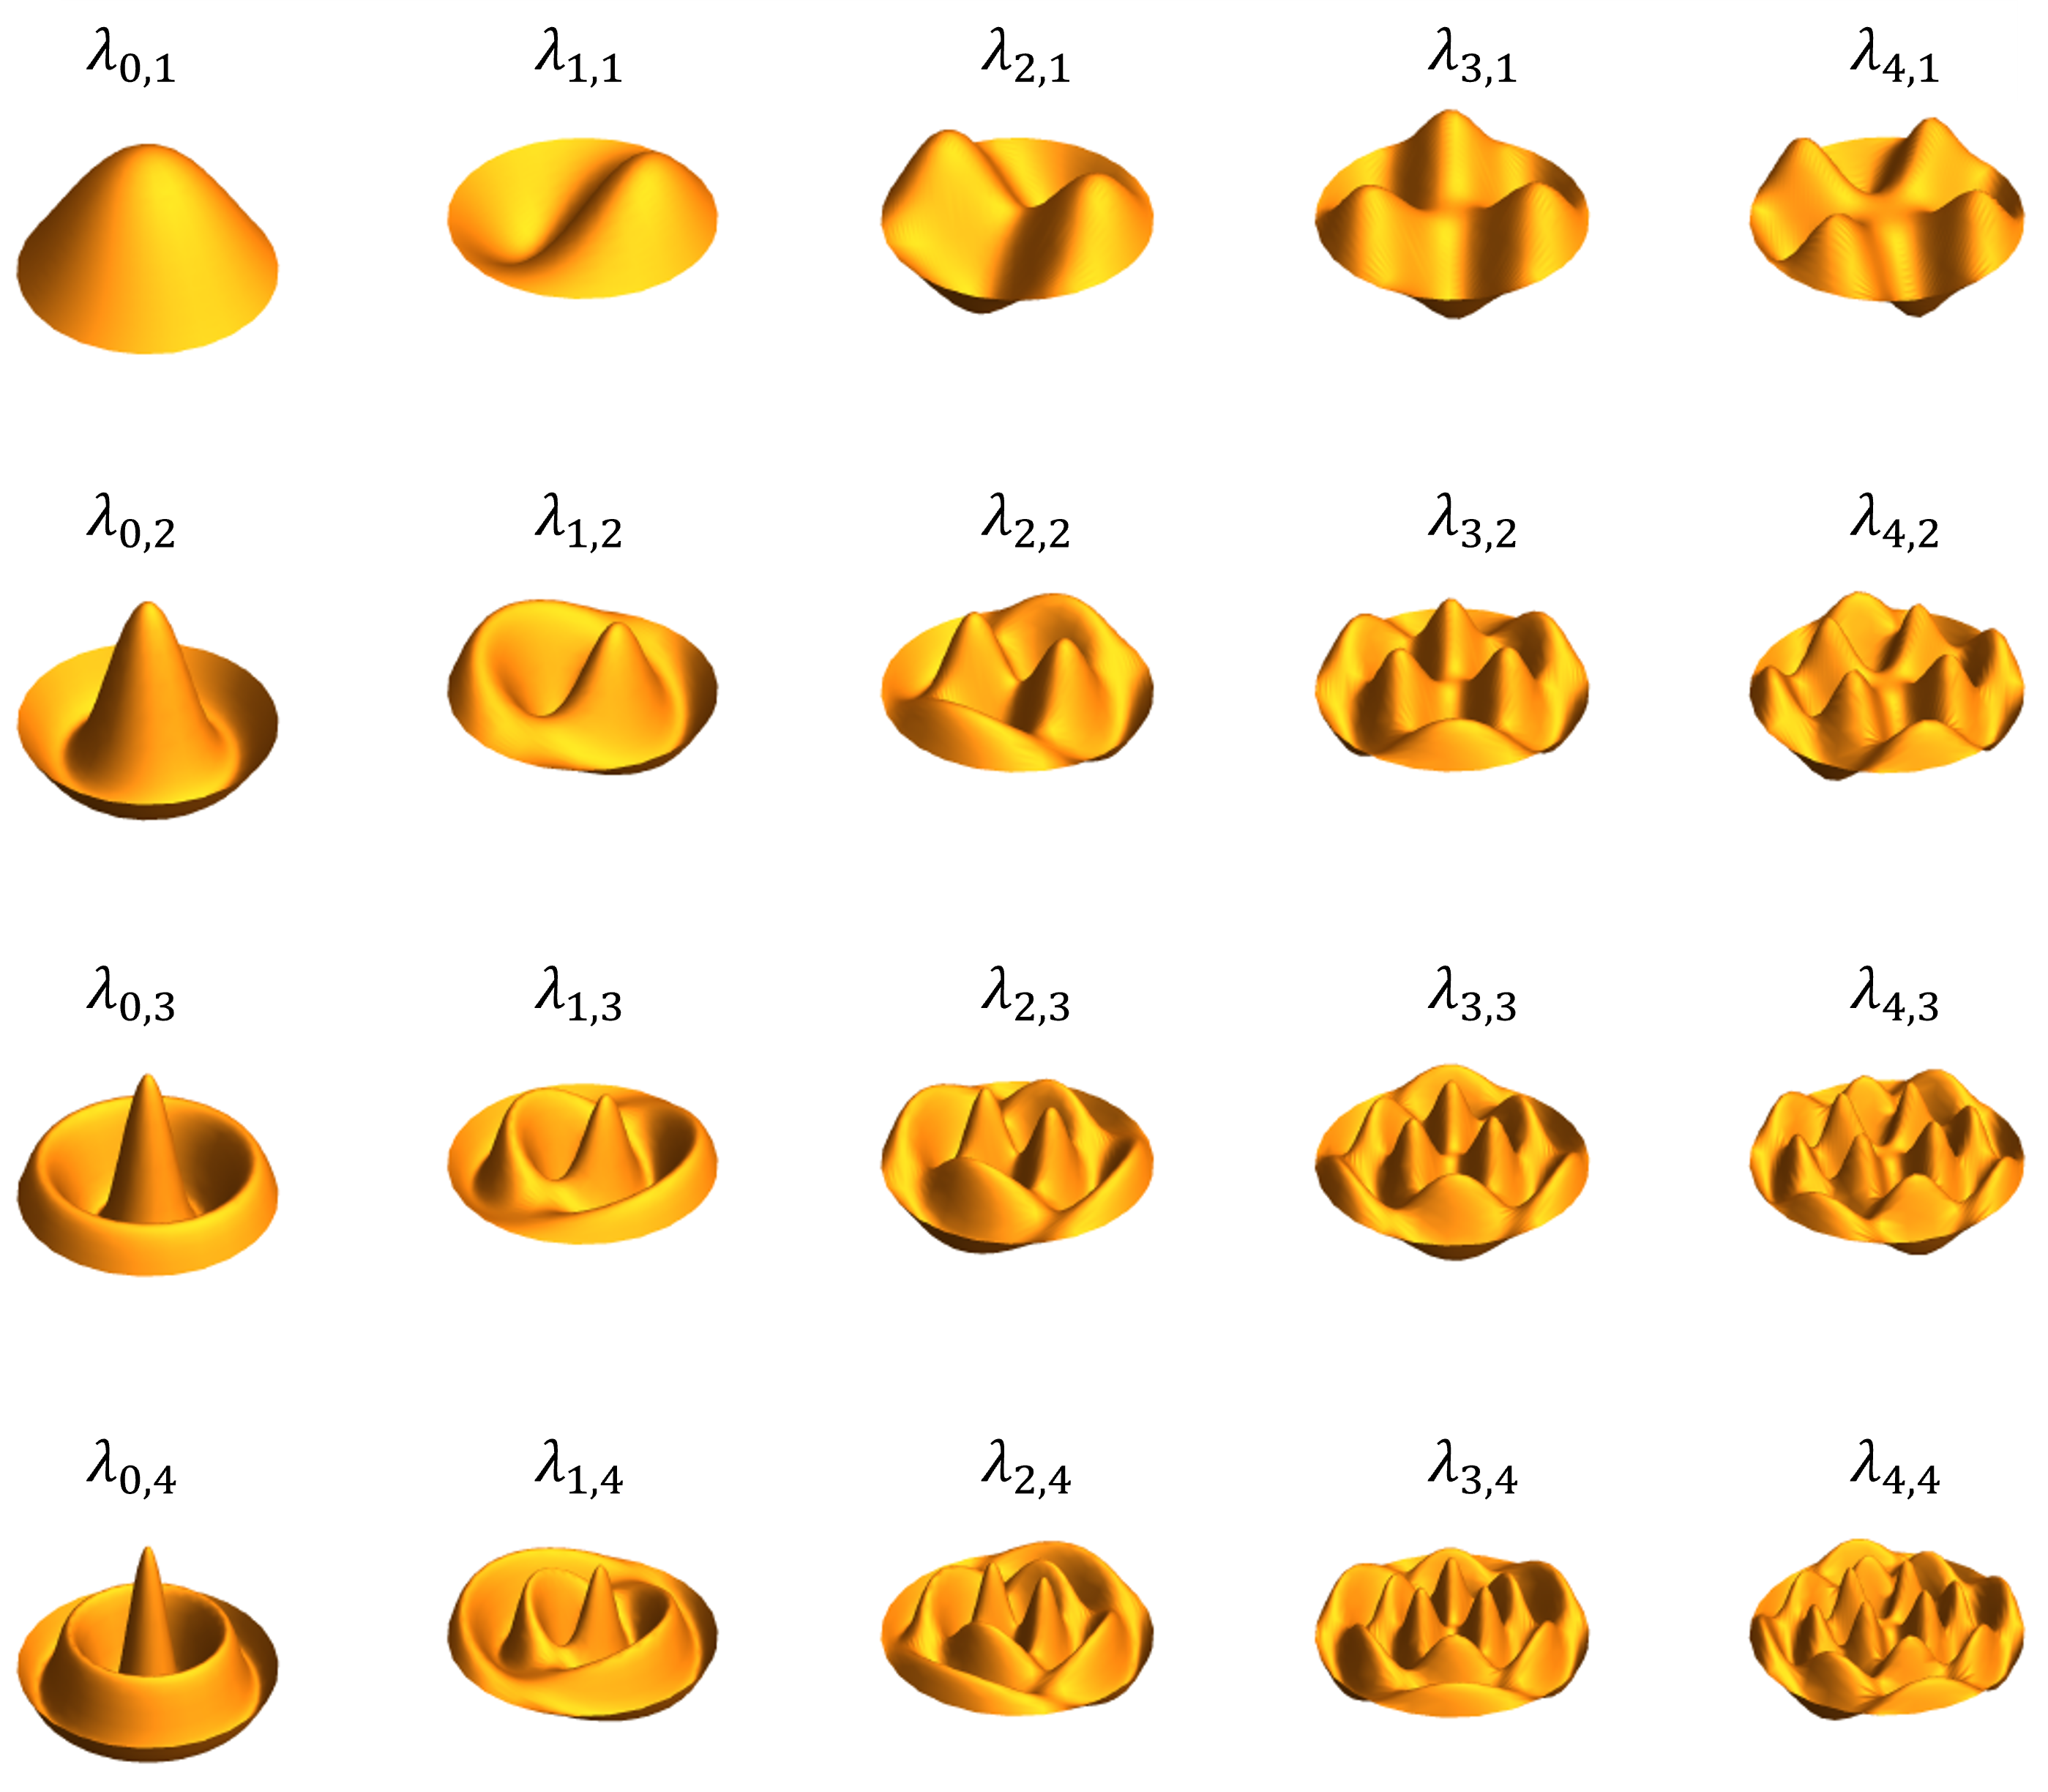
\includegraphics[scale=0.55]{media/Vibrations.png}
    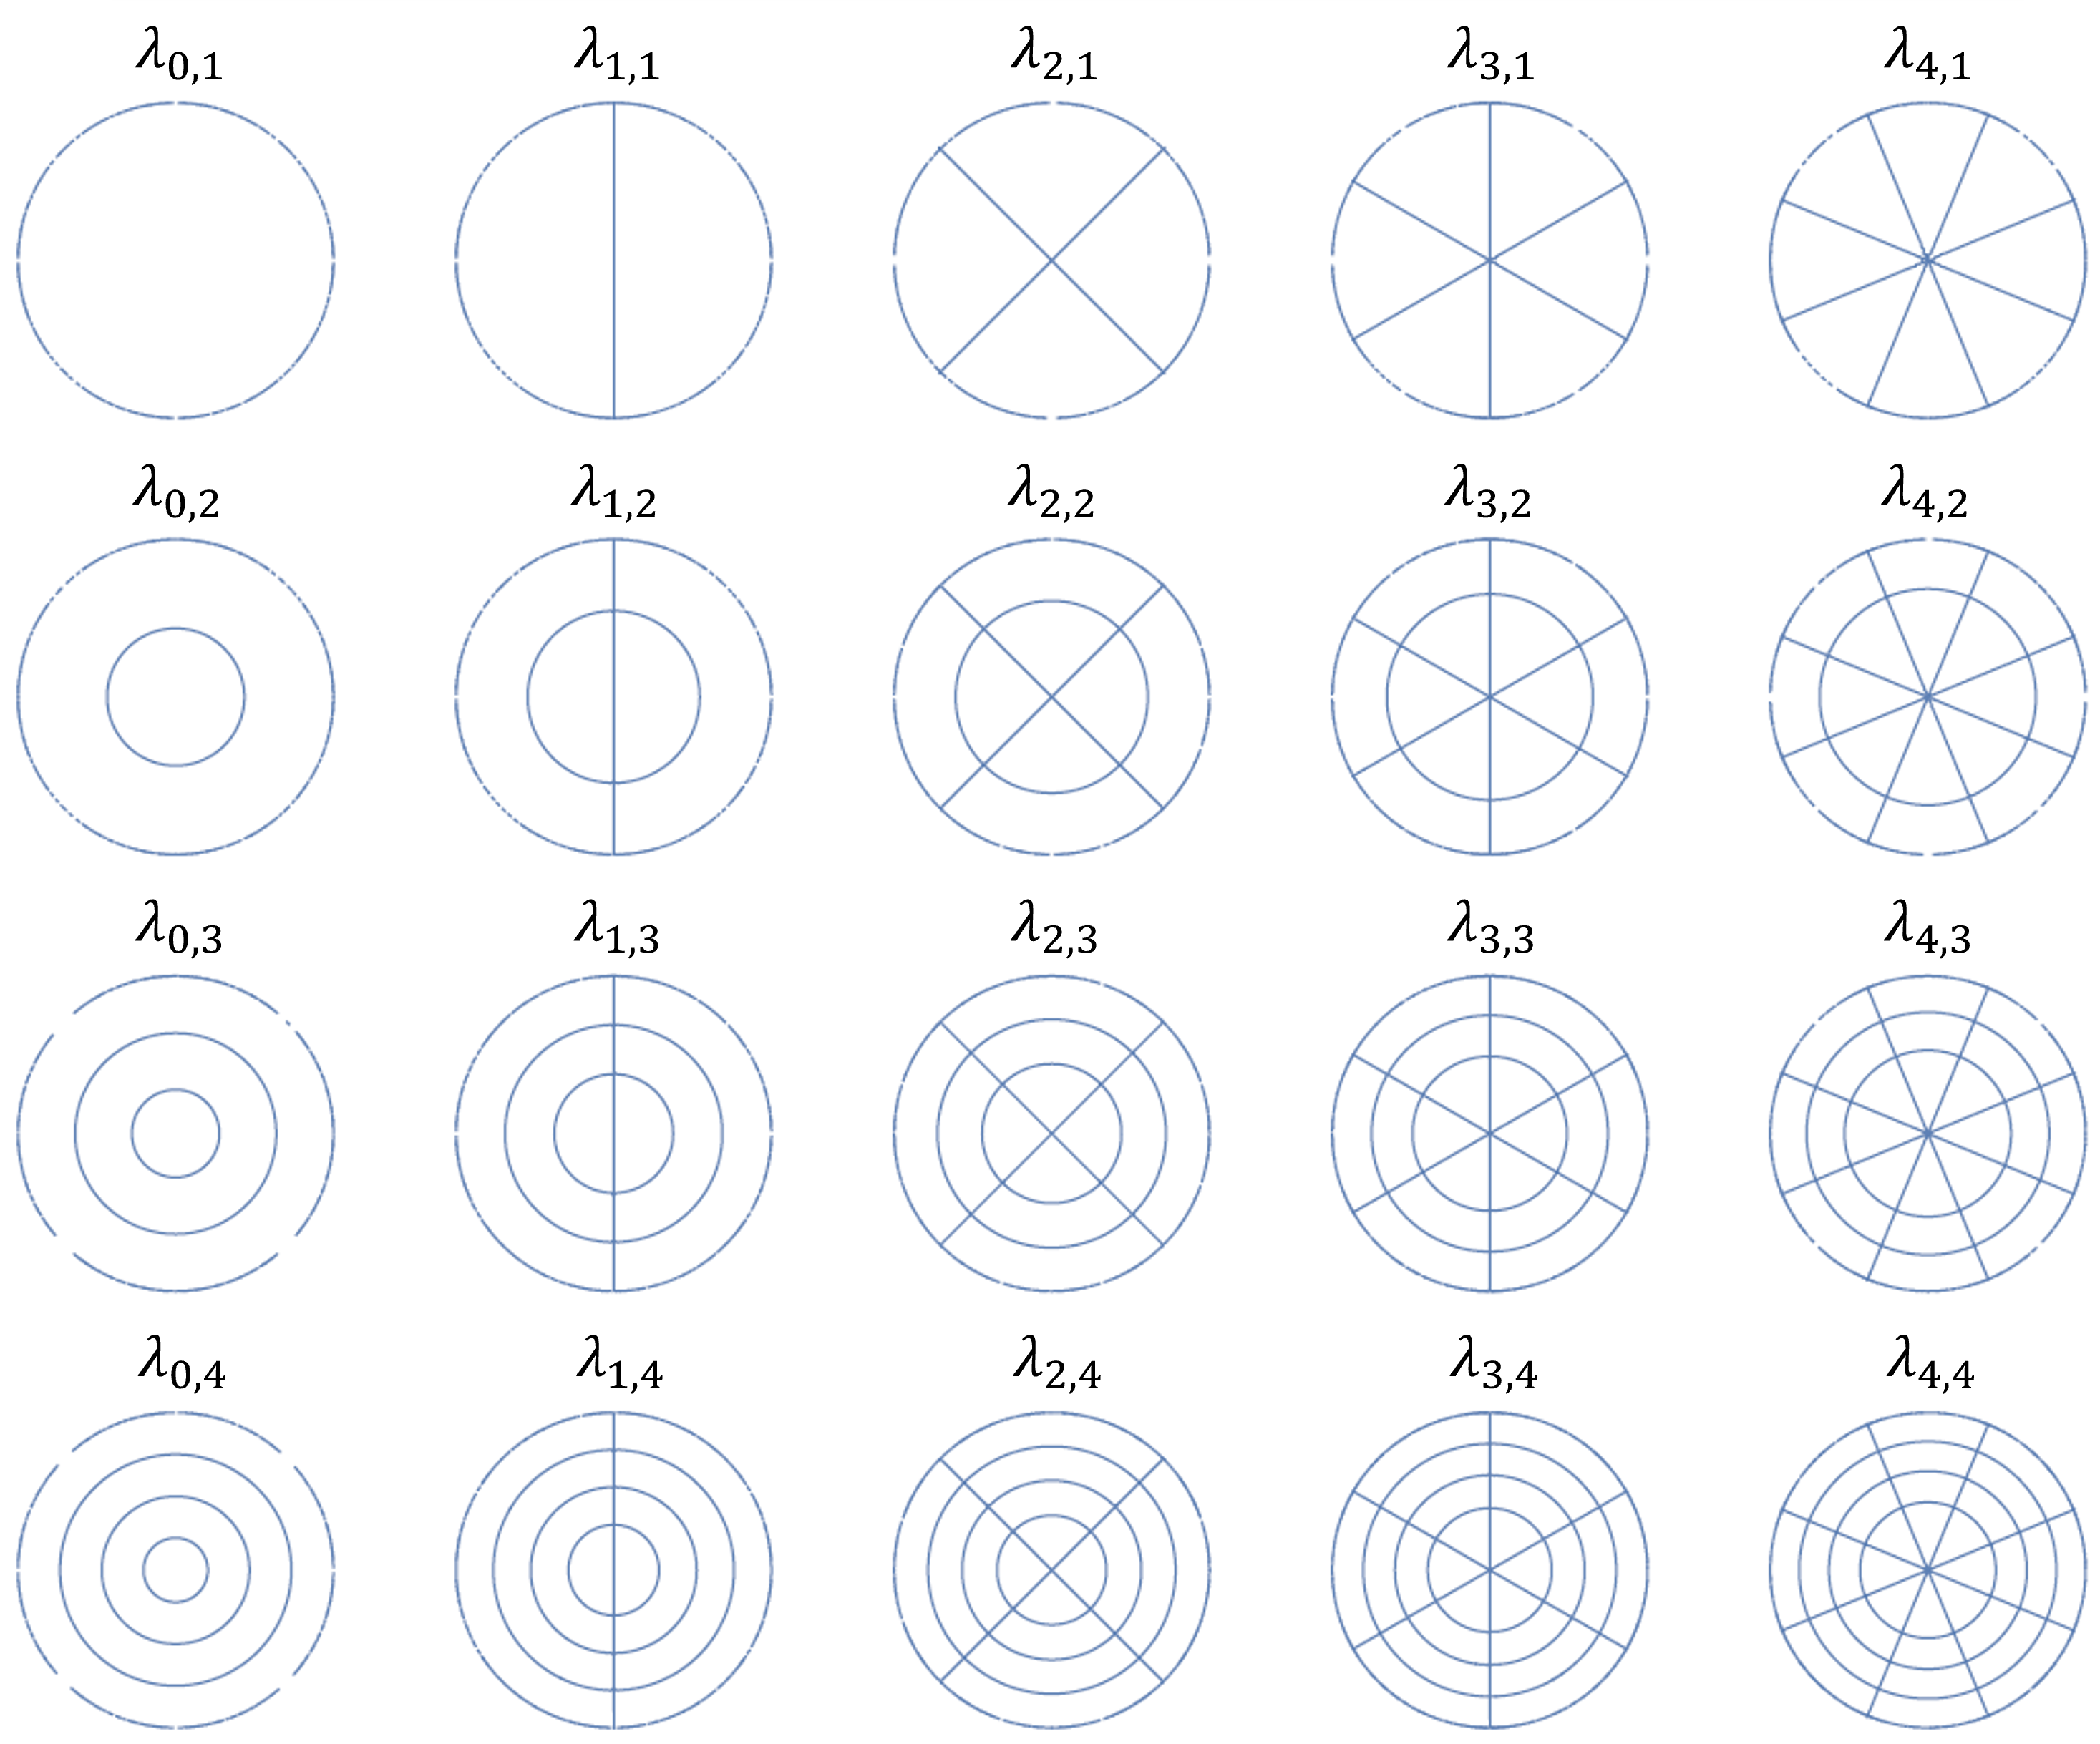
\includegraphics[scale=0.55]{media/Nodes.png}
    \caption{The whole solution is a linear combination of standing waves. The fundamental vibrations (top) are shown for radially derelict boundary conditions ($\phi(r=R, \theta, t) = 0$) \cite{NDSU_notes}. The nodal curves (bottom) show the set for points for which $\phi(r, \theta) = 0 \, \forall t$, dividing the domain into nodal regions \cite{NDSU_notes}. Recall that that $\lambda_{n,m}$ is the eigenmode for the $m$-th root of the $n$-th order Bessel function $J_n$ for $m = 1, 2, 3, 4$.}
\end{center}
\end{figure}

% %%%%%%%%%%%%%%%%%%%%%%%%%%%%%%%%%%%%%%%%%%%%%%%%%%%%%%%%%%%%%%%%%%%%%%%%
% From Solution .tex file from Hannah
% \begin{exercise}\label{ex:ex3}  Swirling your coffee.

% When ones swirls their coffee, waves on the surface of the fluid are generated by the motion of the walls. For the small deformation of any planar circular elastic material, the surface deformation, $\phi$,  satisfies the wave equation in plane polar coordinate:
% \begin{equation}\label{eq:q3_PDE}
% \qquad \frac{\partial^{2} \phi}{\partial t^{2}} = c^{2}\left[\frac{1}{r} \frac{\partial}{\partial r} r \frac{\partial \phi}{\partial r}+\frac{1}{r^{2}} \frac{\partial^{2} \phi}{\partial \theta^{2}}\right] 
% \end{equation}
% where we choose to define the driving force of the wave motion for a material initially at rest
% through the boundary and initial conditions:
% \begin{gather}
%  \phi(r=R, \theta, t)=A \cos (\omega t) \cos (\theta)\label{eq:q3_bc1} \\ 
%  \phi(r=0, \theta, t) \text{ finite} \\
%  \phi(r, \theta+2 \pi, t)=\phi(r, \theta, t) \\
%  \phi(r, \theta, 0)=0 \\
%  \phi_{t}(r, \theta, 0)=0
% \end{gather}
% Solve for $\phi$ for all $t$, $\theta$ and $r$ using the method of eigenfunction expansions. Also determine whether there is any resonance for any value of $\omega$ and if so what value.

% Steps in the solution:

% a) Complete separation of variables to determine the eigenfunctions for the operator and
% boundary conditions:
% \begin{gather} \nabla^{2} \psi=\left[\frac{1}{r} \frac{\partial}{\partial r} r \frac{\partial \psi}{\partial r}+\frac{1}{r^{2}} \frac{\partial^{2} \psi}{\partial \theta^{2}}\right] =-\lambda \psi \label{eq:q3a_1} \\ 
% \psi(r=R, \theta) =0 \label{eq:q3a_2}\\ 
% \psi(r=0, \theta) \text { finite }\label{eq:q3a_3}\\ 
% \psi(r, \theta+2 \pi)=\psi(r, \theta) \label{eq:q3a_4}\end{gather}

% b) Substract from the solution for $\phi$ a function which makes the boundary conditions homogeneous but perhaps introduces inhomogeneities in the initial conditions and the equation
% itself.

% c) Use the eigenfunctions determined from the separation of variables in the method of
% eigenfunction expansions and solve for $\phi$.

% \end{exercise}

% %%%%%%%%%%%%%%%%%%%%%%%%%%%%%%%%%%%%%%%%%%%%%%%%%%%%%%%%%%%%%%%%%%%%%%%%

% \begin{answer*}
% a) Consider the homogeneous stationary boundary value problem in equations (\ref{eq:q3a_1})-(\ref{eq:q3a_4}). Using separation of variables, assume 
% \begin{equation}
%     \psi(r,\theta) = \mathcal{R}(r)\Theta(\theta).
% \end{equation}
% Then we can rewrite the PDE as 
% \begin{equation}
%     \Theta\frac{1}{r} \frac{d}{d r}\left(r \mathcal{R}^{\prime}\right)+\frac{1}{r^{2}} \mathcal{R} \Theta^{\prime \prime}=-\lambda \Theta\mathcal{R} \implies \frac{1}{\mathcal{R}}  r \frac{d}{d r}\left(r \mathcal{R}^{\prime}\right)+\lambda r^{2}=-\frac{1}{\Theta} \Theta^{\prime \prime} = \alpha^{2}
% \end{equation}
% with $\alpha^{2}$ some constant. First we solve the angular problem: 
% \begin{equation}
%     \Theta^{\prime \prime} = -\alpha^{2}\Theta \implies \Theta(\theta) = a \cos(\alpha \theta) + b \sin(\alpha \theta).
% \end{equation}
% Applying the condition $\psi(r,\theta+2\pi) = \psi(r,\theta)$: 
% \begin{multline}
%     a \cos(\alpha \theta + \alpha 2 \pi ) + b \sin(\alpha \theta+ \alpha 2 \pi) = a \cos(\alpha \theta) + b \sin(\alpha \theta )  \\
%     \implies \cos(\alpha \theta + \alpha 2 \pi ) = \cos(\alpha \theta) \ \ \text{and} \ \ \sin(\alpha \theta + \alpha 2 \pi ) = \sin(\alpha \theta) \implies \alpha_{n} = n \in \mathds{Z}^{\geq 0}
% \end{multline}
% therefore a solution to the angular problem is
% \begin{equation}
%     \Theta_{n}(\theta) = a_{n} \cos(n \theta) + b_{n} \sin(n \theta).
% \end{equation}
% Now we solve the radial problem
% \begin{equation}
%     \frac{1}{\mathcal{R}}  r \frac{d}{d r}\left(r \mathcal{R}^{\prime}\right)+\lambda r^{2} = n^{2} \implies r \frac{d}{d r}\left(r \mathcal{R}^{\prime}\right) + (\lambda r^{2} - n^{2})\mathcal{R} = 0.
% \end{equation}
% The above is in the form of a Bessel equation and therefore the solutions to the radial problem are in the form of Bessel functions of order $n$: 
% \begin{equation}
%     \mathcal{R}(r) = c J_{n}(\sqrt{\lambda} r) + d Y_{n}(\sqrt{\lambda} r).
% \end{equation}
% Applying boundary conditions:
% \begin{gather}
%     \mathcal{R}(0) \text{ finite} \implies d = 0 \\
%     \mathcal{R}(R) = 0 \implies c J_{n}(\sqrt{\lambda_{n,m}} r) = 0 \implies \sqrt{\lambda_{n,m}} R = z_{n,m} 
% \end{gather}
% where $z_{n,m}$ is the $m$-th zero of the $n$-th order Bessel function $J_{n}$. Therefore the eigenfunctions of (\ref{eq:q3a_1}) are of the form 
% \begin{equation}
%     \psi_{n,m} (r,\theta) = \big(a_{nm} \cos(n \theta) + b_{nm} \sin(n \theta)\big) J_{n}(\sqrt{\lambda_{n,m}} r).
% \end{equation}

% b) Now consider the original problem (\ref{eq:q3_PDE}). The boundary condition (\ref{eq:q3_bc1}) is inhomogeneous so we want to rescale the problem to have homogeneous boundary conditions. Let 
% \begin{equation}
%     \Tilde{\phi} = \phi - A \left( \frac{r^{2}}{R^{2}} \right) \cos(\omega t) \cos(\theta)
% \end{equation}
% - note that the $r^{2}/R^{2}$ term is necessary to resolve the singularity from the ODE, you may have tried the transformation without it to see that the term is necessary. Taking time and spatial derivatives of $\Tilde{\phi}$ to rewrite the PDE: 
% \begin{gather}
%     \phi_{t} = \Tilde{\phi}_{t} - A \omega \left( \frac{r^{2}}{R^{2}} \right) \sin(\omega t) \cos(\theta)\\
%      \phi_{tt}  = \Tilde{\phi}_{tt} - A \omega^{2} \left( \frac{r^{2}}{R^{2}} \right) \cos(\omega t) \cos(\theta)\\
%      \phi_{r} = \Tilde{\phi}_{r} + 2 A \left( \frac{r}{R^{2}} \right) \cos(\omega t) \cos(\theta)\\
%      \frac{1}{r}\frac{\partial}{\partial r} (r \phi_{r}) = \frac{1}{r}\frac{\partial}{\partial r} (r \Tilde{\phi}_{r}) + 4A \left( \frac{1}{R^{2}} \right) \cos(\omega t) \cos(\theta) \\
%      \frac{1}{r^{2}} \phi_{\theta \theta} = \frac{1}{r^{2}} \Tilde{\phi}_{\theta \theta} - A \left( \frac{1}{R^{2}} \right) \cos(\omega t) \cos(\theta)
% \end{gather}
% Now we can put it all together to rewrite the problem in terms of the transformed variable $\Tilde{\phi}$: 
% \begin{multline}
%     \Tilde{\phi}_{tt} - A \omega^{2} \left( \frac{r^{2}}{R^{2}} \right) \cos(\omega t) \cos(\theta) = c^{2} \Bigg[ \frac{1}{r}\frac{\partial}{\partial r} (r \Tilde{\phi}_{r}) + 4A \left( \frac{1}{R^{2}} \right) \cos(\omega t) \cos(\theta) \\
%     + \frac{1}{r^{2}} \Tilde{\phi}_{\theta \theta} - A \left( \frac{1}{R^{2}} \right) \cos(\omega t) \cos(\theta)\Bigg]
% \end{multline}
% which simplifies to 
% \begin{equation}
%     \Tilde{\phi}_{tt} - A  \left( \frac{1}{R^{2}} \right) \cos(\omega t) \cos(\theta) (\omega^{2} r^{2} + 3 c^{2}) = c^{2} \left[ \frac{1}{r}\frac{\partial}{\partial r}(r \Tilde{\phi}_{r}) +  \frac{1}{r^{2}} \Tilde{\phi}_{\theta \theta}  \right]
% \end{equation}
% with the initial and boundary conditions 
% \begin{gather}
%     \Tilde{\phi}(r = R, \theta, t) = 0 \\ 
%     \Tilde{\phi}(r = 0, \theta, t) \ \ \text{finite} \\
%     \Tilde{\phi}(r, \theta + 2 \pi, t) = \Tilde{\phi}(r, \theta, t) \\
%     \Tilde{\phi}(r, \theta, 0) = - A\left(\frac{r^{2}}{R^{2}} \right) \cos(\theta) \\ 
%     \Tilde{\phi}_{t} (r, \theta,0) = 0
% \end{gather}
% Note that the boundary conditions are now homogeneous, but one of the initial condition is inhomogeneous. For compactness, define 
% \begin{equation}
%     f(r,\theta,t) =  A  \left( \frac{1}{R^{2}} \right) \cos(\omega t) \cos(\theta) (\omega^{2} r^{2} + 3 c^{2}).
% \end{equation}


% c) To solve the new PDE in $\Tilde{\phi}$ we expand the inhomogeneity $f(r,\theta,t)$ in the eigenfunctions of the stationary problem: 
% \begin{equation}
%     f(r,\theta,t) = \sum_{n = 0}^{\infty} \sum_{m=1}^{\infty}\big(c_{nm}(t) \cos(n \theta) + d_{nm}(t) \sin(n \theta)\big) J_{n}(\sqrt{\lambda_{n,m}} r).
% \end{equation}
% Using orthogonality of eigenfunctions we can solve for $c_{nm}(t),d_{nm}(t)$: 
% \begin{gather}
%     c_{nm}(t) = \frac{\int_{0}^{R} \int_{0}^{2\pi} f(r,\theta,t) r J_{n}(\sqrt{\lambda_{n,m}} r) \cos(n\theta) \ dr \ d\theta}{\int_{0}^{R} \int_{0}^{2\pi} r J_{n}^{2}(\sqrt{\lambda_{n,m}} r) \cos^{2}(n\theta) \ dr \ d\theta} \\
%     d_{nm}(t) = \frac{\int_{0}^{R} \int_{0}^{2\pi} f(r,\theta,t) r J_{n}(\sqrt{\lambda_{n,m}} r) \sin(n\theta) \ dr \ d\theta}{\int_{0}^{R} \int_{0}^{2\pi} r J_{n}^{2}(\sqrt{\lambda_{n,m}} r) \sin^{2}(n\theta) \ dr \ d\theta}.
% \end{gather}
% Computing some of the integrals:
% \begin{equation}
%     \int_{0}^{R} \int_{0}^{2\pi} r J_{n}^{2}(\sqrt{\lambda_{n,m}} r) \cos^{2}(n\theta) \ dr \ d\theta = \frac{1}{2}\pi R^{2} J_{n+1}^{2}(\sqrt{\lambda_{n,m}} R)
% \end{equation}
% We can rewrite
% \begin{multline}
%     \int_{0}^{R} \int_{0}^{2\pi} f(r,\theta,t) r J_{n}(\sqrt{\lambda_{n,m}} r) \cos(n\theta) \ dr \ d\theta \\
%     = \frac{A}{R^{2}} \cos( \omega t)\left[\int_{0}^{2 \pi} \cos (\theta) \cos (n \theta) d \theta \int_{0}^{R}\left(\omega^{2} r^{2}+3 c^{2}\right) r J_{n}\left(\sqrt{\lambda_{n, m}} r\right) d r\right] \label{eq:q1bint}
% \end{multline}
% Notice that 
% \begin{equation}
%     \int_{0}^{2 \pi} \cos (\theta) \cos (n \theta) d \theta = \begin{cases} \pi \ \text{if } n = 1\\ 0  \ \text{if } n \neq 1 \end{cases}
% \end{equation}
% and so $c_{nm}(t)$ simplifies to 
% \begin{equation}
%     c_{nm}(t) = \begin{cases} 0 \ \ \ \ \ \ \ \ \ \ \ \ \ \ \ \ \ \ \ \ \ \ \ \ \ \ \ \ \ \ \ \ \ \ \ \ \ \ \ \ \ \ \ \ \ \text{if } n \neq 1 \\ \frac{2 A}{R^{4}} \cos(\omega t) \frac{\int_{0}^{R}\left(w^{2} r^{2}+3 c^{2}\right) r J_{1}\left(\sqrt{\lambda_{1 m}} r\right) d r}{J_{2}^{2}\left(\sqrt{\lambda_{1 m}} R\right)} \ \ \ \text{if } n = 1\end{cases}
% \end{equation}
% Note that 
% \begin{equation}
%     \int_{0}^{2\pi} \sin(n\theta) \cos(\theta) d\theta = 0 \ \ \forall n
% \end{equation}
% which means that 
% \begin{equation}
%     d_{nm}(t) = 0.
% \end{equation}
% So we find that 
% \begin{equation}
%     f(r,\theta,t) = \frac{2 A}{R^{4}} \cos(\omega t) \sum_{m=1}^{\infty}  \frac{\int_{0}^{R}\left(w^{2} \zeta^{2}+3 c^{2}\right) \zeta J_{1}\left(\sqrt{\lambda_{1 m}} \zeta\right) d\zeta}{J_{2}^{2}\left(\sqrt{\lambda_{1 m}} R\right)} \cos(\theta) J_{1}(\sqrt{\lambda_{n,m}}r)
% \end{equation}
% or if we non-dimensionalize the variable in the integral with $R\eta = \zeta$
% \begin{equation}
%     f(r,\theta,t) = \frac{2 A}{R^{2}} \cos(\omega t) \sum_{m=1}^{\infty}  \frac{\int_{0}^{1}\left(w^{2} \eta^{2}+3 c^{2}\right) \eta J_{1}\left(\sqrt{\lambda_{1 m}} R\eta\right) d\eta}{J_{2}^{2}\left(\sqrt{\lambda_{1 m}} R\right)} \cos(\theta) J_{1}(\sqrt{\lambda_{n,m}}r).
% \end{equation}
% Now we can write down the eigenfunction expansion of $\Tilde{\phi}(r,\theta,t)$: 
% \begin{equation}
%     \Tilde{\phi}(r,\theta,t) = \sum_{n = 0}^{\infty} \sum_{m = 1}^{\infty }\big(a_{nm}(t) \cos(n \theta) + b_{nm}(t) \sin(n \theta)\big) J_{n}(\sqrt{\lambda_{n,m}} r)
% \end{equation}
% Then we can deduce the following relationships from the PDE: 
% \begin{align}
%     &n \neq 1: a_{nm}''(t) = -\lambda_{n,m}c^{2} a_{nm}(t)\\
%     &n = 1: a_{1m}''(t) - c_{1m}(t) = -\lambda_{1,m}c^{2} a_{1m}(t) \\
%     & \forall \ n: \ \ \ b_{nm}''(t) = -\lambda_{n,m}c^{2} b_{nm}(t) 
% \end{align}
% Now we can use the initial conditions for the PDE to get initial conditions for these coefficient ODEs: 
% \begin{equation}
%     \Tilde{\phi}(r, \theta, 0) = - A\left(\frac{r^{2}}{R^{2}} \right) \cos(\theta) = \sum_{n = 0}^{\infty} \sum_{m = 1}^{\infty }\big(a_{nm}(0) \cos(n \theta) + b_{nm}(0) \sin(n \theta)\big) J_{n}(\sqrt{\lambda_{n,m}} r)
% \end{equation}
% We note that the initial condition does not have a $\sin(\theta)$ term and therefore 
% \begin{equation}
%     b_{nm}(0) = 0. 
% \end{equation}
% To solve for $a_{nm}(0)$ we use orthogonality of eigenfunctions and take inner products of both sides with $\cos(n \theta) J_{n}(\sqrt{\lambda_{n,m}}r)$: 
% \begin{multline}
%     a_{nm}(0) = \frac{\int_{0}^{R} \int_{0}^{2\pi} -A \left(\frac{r}{R}\right)^{2} \cos(\theta) r J_{n}(\sqrt{\lambda_{n,m}} r) \cos(n\theta) \ dr \ d\theta}{\int_{0}^{R} \int_{0}^{2\pi} r J_{n}^{2}(\sqrt{\lambda_{n,m}} r) \cos^{2}(n\theta) \ dr \ d\theta} \\
%     = \frac{\int_{0}^{R} -A \left(\frac{r}{R}\right)^{2} r J_{n}(\sqrt{\lambda_{n,m}} r)dr \int_{0}^{2\pi}\cos(\theta)  \cos(n\theta) \  d\theta}{\pi R^{2} \frac{1}{2} J_{2}^{2}(\sqrt{\lambda_{n,m}} R)} \\
%     = \begin{cases} 0 \ \ \ \ \ \ \ \ \ \ \ \ \ \ \ \ \ \ \ \ \ \ \ \ \ \ \ \ \ \ \ \ \ \ \ \ \ \ \ \ \ \ \ \ \ \ \ \ \ \  \text{if } n \neq 1 \\
%     - \frac{2A}{R^{4}J_{n+1}^{2}(\sqrt{\lambda_{1,m}} R)}\int_{0}^{R} r^{3} J_{1}(\sqrt{\lambda_{1,m}} r) dr \ \ \ \ \ \text{if } n = 1\end{cases} \\
%     = \begin{cases} 0 \ \ \ \ \ \ \ \ \ \ \ \ \ \ \ \ \ \ \ \ \ \ \ \ \ \ \ \ \ \ \ \ \ \ \ \ \ \ \ \ \ \ \ \ \ \ \ \ \ \  \text{if } n \neq 1 \\
%     - \frac{2A}{J_{2}^{2}(\sqrt{\lambda_{1,m}} R)}\int_{0}^{1} \eta^{3} J_{1}(\sqrt{\lambda_{1,m}} R  \eta) d\eta \ \ \ \ \ \text{if } n = 1\end{cases}
% \end{multline}
% The second initial condition tells us that 
% \begin{equation}
%     \Tilde{\phi}_{t} (r, \theta,0) =\sum_{n = 0}^{\infty} \sum_{m = 1}^{\infty }\big(a'_{nm}(0) \cos(n \theta) + b'_{nm}(0) \sin(n \theta)\big) J_{n}(\sqrt{\lambda_{n,m}} r)  = 0
% \end{equation}
% which implies that 
% \begin{equation}
%     a_{nm}'(0) = 0, \ \ \ \ b_{nm}'(0) = 0.
% \end{equation}
% Now we can solve the ODEs for $a_{nm},b_{nm}$. First we consider $n \neq 1$ with the initial conditions: 
% \begin{equation}
%     a_{nm}(t) = K_{1} \cos(c \sqrt{\lambda_{n,m}} t) + K_{2} \sin(c \sqrt{\lambda_{n,m}} t) \implies K_{1} = 0, k_{2} = 0 \implies a_{nm}(t) = 0 
% \end{equation}
% Similarly, we find for all $n$ 
% \begin{equation}
%     b_{nm}(t) = 0.
% \end{equation}
% Now we consider the case $n = 1$: 
% \begin{equation}
%     a''_{nm} -\frac{2 A}{R^{2}} \cos(\omega t)  \frac{\int_{0}^{1}\left(w^{2} \eta^{2}+3 c^{2}\right) \eta J_{1}\left(\sqrt{\lambda_{1 m}} R\eta\right) d\eta}{J_{2}^{2}\left(\sqrt{\lambda_{1 m}} R\right)} = - c^{2} \lambda_{n,m} a_{1m} 
% \end{equation}
% The homogeneous solution to this ODE is of the form 
% \begin{equation}
%     a_{1m}^{h}(t) = K_{3} \cos(c \sqrt{\lambda_{n,m}} t) + K_{4} \sin(c \sqrt{\lambda_{n,m}} t)
% \end{equation}
% and by inspection we find a particular solution 
% \begin{equation}
%     a_{1m}^{p}(t) = K_{5} \cos(\omega t)
% \end{equation}
% where 
% \begin{equation}
%     K_{5} = \frac{1}{c^{2} \lambda_{n,m} - \omega^{2}} \frac{2 A}{R^{2}}   \frac{\int_{0}^{1}\left(w^{2} \eta^{2}+3 c^{2}\right) \eta J_{1}\left(\sqrt{\lambda_{1, m}} R\eta\right) d\eta}{J_{2}^{2}\left(\sqrt{\lambda_{1, m}} R\right)} 
% \end{equation}
% and so putting it all together, the general solution for the coefficients is
% \begin{multline}
%     a_{1m}(t) = K_{3} \cos(c \sqrt{\lambda_{n,m}} t) + K_{4} \sin(c \sqrt{\lambda_{n,m}} t) \\
%     + \frac{1}{c^{2} \lambda_{n,m} - \omega^{2}} \frac{2 A}{R^{2}}   \frac{\int_{0}^{1}\left(w^{2} \eta^{2}+3 c^{2}\right) \eta J_{1}\left(\sqrt{\lambda_{1, m}} R\eta\right) d\eta}{J_{2}^{2}\left(\sqrt{\lambda_{1, m}} R\right)}  \cos(\omega t)
% \end{multline}
% Furthermore from the initial conditions we find that 
% \begin{gather}
%     K_{4} = 0 
% \end{gather}
% \begin{multline}
%     K_{3} =  - \frac{2A}{J_{2}^{2}(\sqrt{\lambda_{1,m}} R)}\int_{0}^{1} \eta^{3} J_{1}(\sqrt{\lambda_{1,m}} R  \eta) d\eta \\
%     -\frac{1}{c^{2} \lambda_{n,m} - \omega^{2}} \frac{2 A}{R^{2}}   \frac{\int_{0}^{1}\left(w^{2} \eta^{2}+3 c^{2}\right) \eta J_{1}\left(\sqrt{\lambda_{1, m}} R\eta\right) d\eta}{J_{2}^{2}\left(\sqrt{\lambda_{1, m}} R\right)}
% \end{multline}
% So finally we have a solution: 
% \begin{multline}
%     \Tilde{\phi}(r,\theta,t) = \sum_{m =1}^{\infty } \Bigg(\frac{1}{c^{2} \lambda_{n,m} - \omega^{2}} \frac{2 A}{R^{2}}   \frac{\int_{0}^{1}\left(w^{2} \eta^{2}+3 c^{2}\right) \eta J_{1}\left(\sqrt{\lambda_{1, m}} R\eta\right) d\eta}{J_{2}^{2}\left(\sqrt{\lambda_{1, m}} R\right)} \cos(\omega t) \\
%      - \frac{2A}{J_{2}^{2}(\sqrt{\lambda_{1,m}} R)} \Bigg(\int_{0}^{1} \eta^{3} J_{1}(\sqrt{\lambda_{1,m}} R  \eta) d\eta 
%    \\
%    +\frac{1}{c^{2} \lambda_{n,m} - \omega^{2}} \frac{1}{R^{2}}   \int_{0}^{1}\left(w^{2} \eta^{2}+3 c^{2}\right) \eta J_{1}\left(\sqrt{\lambda_{1, m}} R\eta\right) d\eta \Bigg) \cos(c \sqrt{\lambda_{1,m}} t) \Bigg) \cos(\theta) J_{1} (\sqrt{\lambda_{1,m}} r)
% \end{multline}
% and the solution in the original variable 
% \begin{equation}
%     \phi(r,\theta,t) = A \Big( \frac{r}{R}\Big)^{2}  \cos(\omega t) \cos(\theta) + \Tilde{\phi}(r,\theta,t)
% \end{equation}
% \end{answer*}


\end{document}